%%
%% DOCUMENT TYPE
%%

% general options:
% - inputenc        file encoding (should be "utf8" in most cases)
% - de/en           language of your work (influence pre-defined tokens)
% - declaration     adds the mandatory statutory declaration for theses
% - abstract        adds the abstract (from file "prelude_abstract.tex")
% - acknowledgment  adds an acknowledgment (from file "prelude_acknowledgment.tex")
%                   it is a nice gesture to personally thank people who
%                   supported you during your work.
% - symbollist      adds a list of symbols (from file "prelude_symbols.tex")
% - figurelist      adds and automatically creates a list of figures 
% - tablelist       adds and automatically creates a list of tables
% - index           generates an index based on the package "makeidx", please
%                   refer to its documentation for usage on index markup
% - bibbacklinks    adds backlinks from bibliography to the pages, where the
%                   corresponding entry is used (cited)
% - gray            make a gray-style version of the thesis report
%
% PhD thesis specific options
% - cv              adds your cv
% - publishsize     changes the page size from A4 to A5 for print publishing
%                   (please change the font size to 9pt, if you use this option)
% - approved        use this option, after your thesis has been formally approved
%                   (this will change the front page to meet formal/legal requirements)
% - ownpub          adds a second bibliography (from file "ownpub.bib") for your own
%                   publications related to the PhD thesis. According to the latest
%                   examination regulations, own work should be part of the regular
%                   bibliography (this option is hence obsolete)

\documentclass[en,print,inputenc=utf8]{tuhhthesis}
\usepackage{tuhhlistings}
\usepackage{multirow}
\usepackage{siunitx}

%%
%% SETUP BLOCK
%%

% thesis type, must be one of the following
% - projectwork
% - bachelorthesis
% - masterthesis
% - diplomathesis
% - phdthesis
\setthesistype{projectwork}

% your full name as printed on any official document (e.g., passport)
\author{Sergej Keller}

% the official title of your work (*must* match the filed title)
\title{Orthogonal Codes for Acoustic Underwater Localization}

% the institution of the first examiner (refer to tuhhlangnames.def)
\institute{InstAutonomousCPS}

% date of submission as DD.MM.YYYY
\submitdate{31.01.2023}

% your matriculation number (for anything but PhD thesis)
\matrnumber{50484}

% PhD thesis only
%\setSexOfAuthor{male}
%\setBirthplace{Hamburg, Deutschland}
%\setPhDType{ing}

% your course of studies
\course{Informatik-Ingenieurwesen}

% full name and affiliation of first and second examiner
\examinerFirst{Prof. Dr.-Ing. Bernd-Christian Renner}{Institute of Autonomous Cyber-Physical Systems\newline Hamburg University of Technology}
%\examinerSecond{Prof. Dr. Volker Turau}{Institute of Telematics\newline Hamburg University of Technology}

\supervisorFirst{Fabian Steinmetz}{Institute of  Autonomous Cyber-Physical Systems, Hamburg University of Technology}
%\supervisorSecond{Volker Turau}{Institute of Telematics, Hamburg University of Technology}

% optional: print the TUB document number on title page
% this only applies, if the document is formally publish under
% a TUB document number
%\tubdoknumber{4711}


% Curriculum Vitae
% only needed for thesis type PhD
%\usepackage[]{currvita}
%\setlength{\cvlabelwidth}{50mm}
%\renewcommand*{\cvlistheadingfont}{\normalfont\sffamily\large\color{tuhh_blue}}
%\renewcommand*{\cvlabelfont}{\normalfont\rmfamily\normalsize\color{tuhh_darkgray}}



%%
%% CONTENT AREA
%%

% mathematical symbols
% absolute value, ceiling, floor
\newcommand{\abs}[1]{\left|{#1}\right|}
\newcommand{\floor}[1]{\left\lfloor{#1}\right\rfloor}
\newcommand{\ceil}[1]{\left\lceil{#1}\right\rceil}

% regular sets %
\newcommand{\setN}{{\mathbb N}}
\newcommand{\setZ}{{\mathbb Z}}
\newcommand{\setQ}{{\mathbb Q}}
\newcommand{\setR}{{\mathbb R}}
\newcommand{\setC}{{\mathbb C}}
\newcommand{\classNP}{{\cal {NP}}}
\newcommand{\classP}{{\cal {P}}}

% a node and a sink
\newcommand{\node}{v}
\newcommand{\sink}{\node_{0}}          % sink

% Node Related Sets
\newcommand{\Network}{G}
\newcommand{\setNodes}{{\mathcal V}}% set of nodes
\newcommand{\setLinks}{{\mathcal E}}% set of edges
\newcommand{\setNeighbors}[1]{{\mathcal N}_{#1}}% neighbors
\newcommand{\setTree}{{\mathcal T}}% tree
\newcommand{\setChildren}{{\mathcal C}}%
\newcommand{\setLeafs}{{\mathcal F}}%
\newcommand{\numNodes}{N}%
\newcommand{\numChildren}{C}%

% density
\newcommand{\nodeDensity}{\varrho}

%% EOF



\begin{document}

\chapter{Introduction}
\section{Motivation}
\section{Setup}
\section{Principle}
\chapter{PN and orthogonal sequences}

To attain a higher level of localization accuracy, there are two primary goals that must be pursued.\\
First, the code used for underwater localization should have an auto-correlation function that approaches a Dirac impulse. This is important because it allows for more efficient detection through the use of correlation techniques.\\
The second factor to consider is the cross-correlation properties of the code. It is essential that these attributes meet certain criteria in order to improve separation from other sequences. Mathematically speaking, this means that the codes should be orthogonal to each other, or at least approaching orthogonality. This will be particularly useful in real-world scenarios where noise, reflections, and other artifacts may be present.\\
In summary, by striving to achieve both of these objectives, it is possible to significantly improve the localization accuracy.

\section{Pseudo-random codes}

There are a couple of techniques to generate PN sequences. Most of these methods use linear feedback shift registers to generate the codes by an initial condition or seed value. In this project I will concertize my research on gold codes, kasami codes and the basic m-sequences which are used for generating gold codes. These types are all based on linear shift registers.\\
M-sequences are defined as binary PN codes, which are generated by linear shift registers with feedback. The sequences are periodic, and contain an equal number of zeros and ones \cite{proakis08}. 
Maximum length sequences need to fulfill certain criteria.  First its length is defined by $N=2^n - 1$ where $n$ is the maximum degree of the generator polynomial $f(X)$ \cite{sarwate80}.
 \begin{equation}
	 \lvert u\rvert=2^n-1=N,~~~\text{from polynomial}~~h(x) \text{of degree}~~n
\end{equation}
\begin{equation}
	\dfrac{N}{gcd(N,q)=N},~~~\text{from decimation polynomials}~~\widetilde{h(x)}
\end{equation}
Second the cross-correlation between m-sequences must take three values only, which are $-1$, $-t(n)$, $t(n) - 2$. With it $t(n)$ is defined by $1+2^{\lfloor0.5(n+2)\rfloor}$ \cite{sarwate80}.
If every pair of m-sequences is a preferred pair, they form a maximal connected set and these sets have a limited carnality. Experiments from Gold and Koptizke showed that the number of such connected pairs is limited. Between degrees $$$$ \cite{gold65}. To get an m-sequence we need a primitive polynomial. 

%\fignoframe{images/lfsr}{Basic structure of an LFSR (Linear Feedback Register). \cite{proakis08}}{fig:framelessFigures}

\subsection{Gold Codes}

Because of not optimal cross-correlation properties m-sequences alone are not applicable for the project. But if these type of codes are combined their correlation qualities can change. Gold Codes are m-sequences where two of them with same length are modulo-2 summed. \cite{proakis08} \\
Recent research shows that some gold codes have high similarity to a Gaussian random variable \cite{merrifield}. 

\begin{equation}
Gold(u,v)=\{u,v,u\oplus v,u\oplus(v \ll1),\dots,u\oplus(v\ll N-1)\}
\end{equation}

%\fignoframe{images/gold}{LFSR structure of preferred generator polynomial of degree 13. \cite{merrifield}}{fig:framelessFigures}

\subsection{Kasami Codes}

Kasami sequences are constructed in the similar fashion by using m-sequences with the exception that a second sequence, which is used in the modulo sum, is formed by decimating the default m-sequence by  $2^{m/2}$ \cite{proakis08} \cite{sarwate80} \cite{peterson72}. Thus, only one generator polynomial is required.

\begin{equation}
w=u[2^{N/2}+1]=\{u_1,\dots, u_i, \dots,u_{N}|\text{take every }i\text{-th bit of u}\} 
\end{equation}
\begin{equation}
Kasami(u)=\{u,u\oplus w,u\oplus(w \ll1),\dots,u\oplus(w\ll2^{N/2}-2)\}
\end{equation}


\section{Comparison}


For the localization process by orthogonal codes certain criteria needs to be met, which were named in the first chapter. To compare the before explained code types three measures are introduced. \\ 
The first one is the peak to side-lobe ratio (PSR) \ref{eq:psr}. This measure is defined by subtracting the mean from the peak of the auto-correlation. Then this value get divided by the standard deviation of the same auto-correlation. A higher PSR value signifies a lower error between the auto correlation and the perfect Dirac resulting in better detection capability. The second one is the ratio between the auto-correlation peak and the maximum of the cross-correlation (ACR) \ref{eq:acr}. There a higher value indicates good code separation qualities.\\
The comparison is done by sampling pairs at degrees six to ten $N$ times from the set of random sequences. These pairs are then used for generating the wanted pseudo-random codes like gold or kasami. Afterwards for all three code types the shown measures are applied.  

%The last one is the correlation coefficient showing if there are similar anchros \ref{eq:coeff}, which would be a bad indicator.

\begin{equation}
PSR=\dfrac{max\{x_{ac}\}-\overline{x_{ac}}}{\sigma_{ac}}
\label{eq:psr}
\end{equation}

\begin{equation}
ACR=\dfrac{max\{x_{ac}\}}{max\{{x_{cc}\}}}
\label{eq:acr}
\end{equation}

%\begin{equation}
%\rho(a1,a2)=\dfrac{cov\{a1,a2\}}{\sigma_{a1}\cdot\sigma_{a2}}
%\label{eq:coeff}
%\end{equation}
%\begin{figure}[h]
%	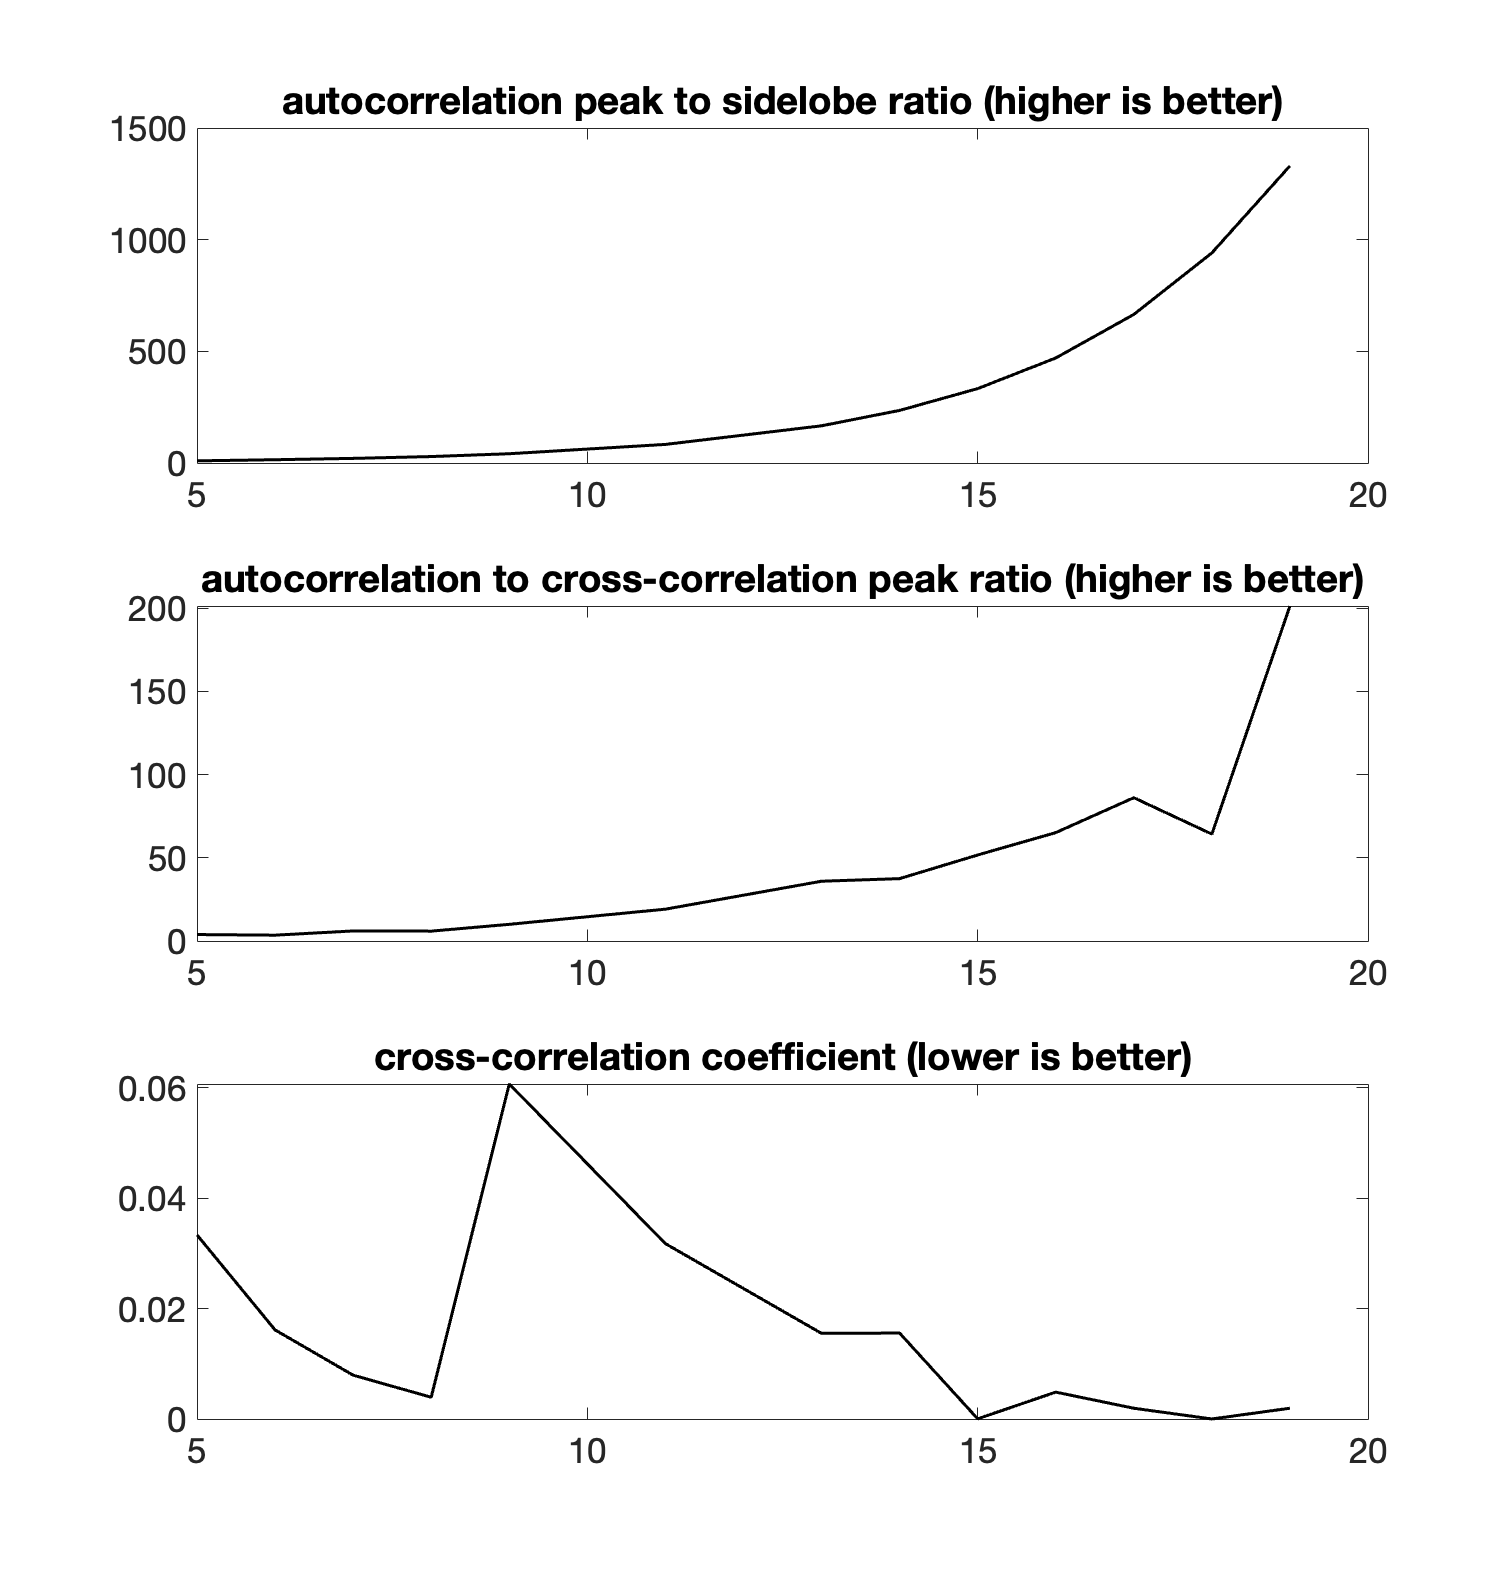
\includegraphics[width=8cm]{images/matlabplots/mseq}
%
%	\caption{Maximum Length Sequence evaluation}
%\end{figure}
%
%\begin{figure}[h]
%	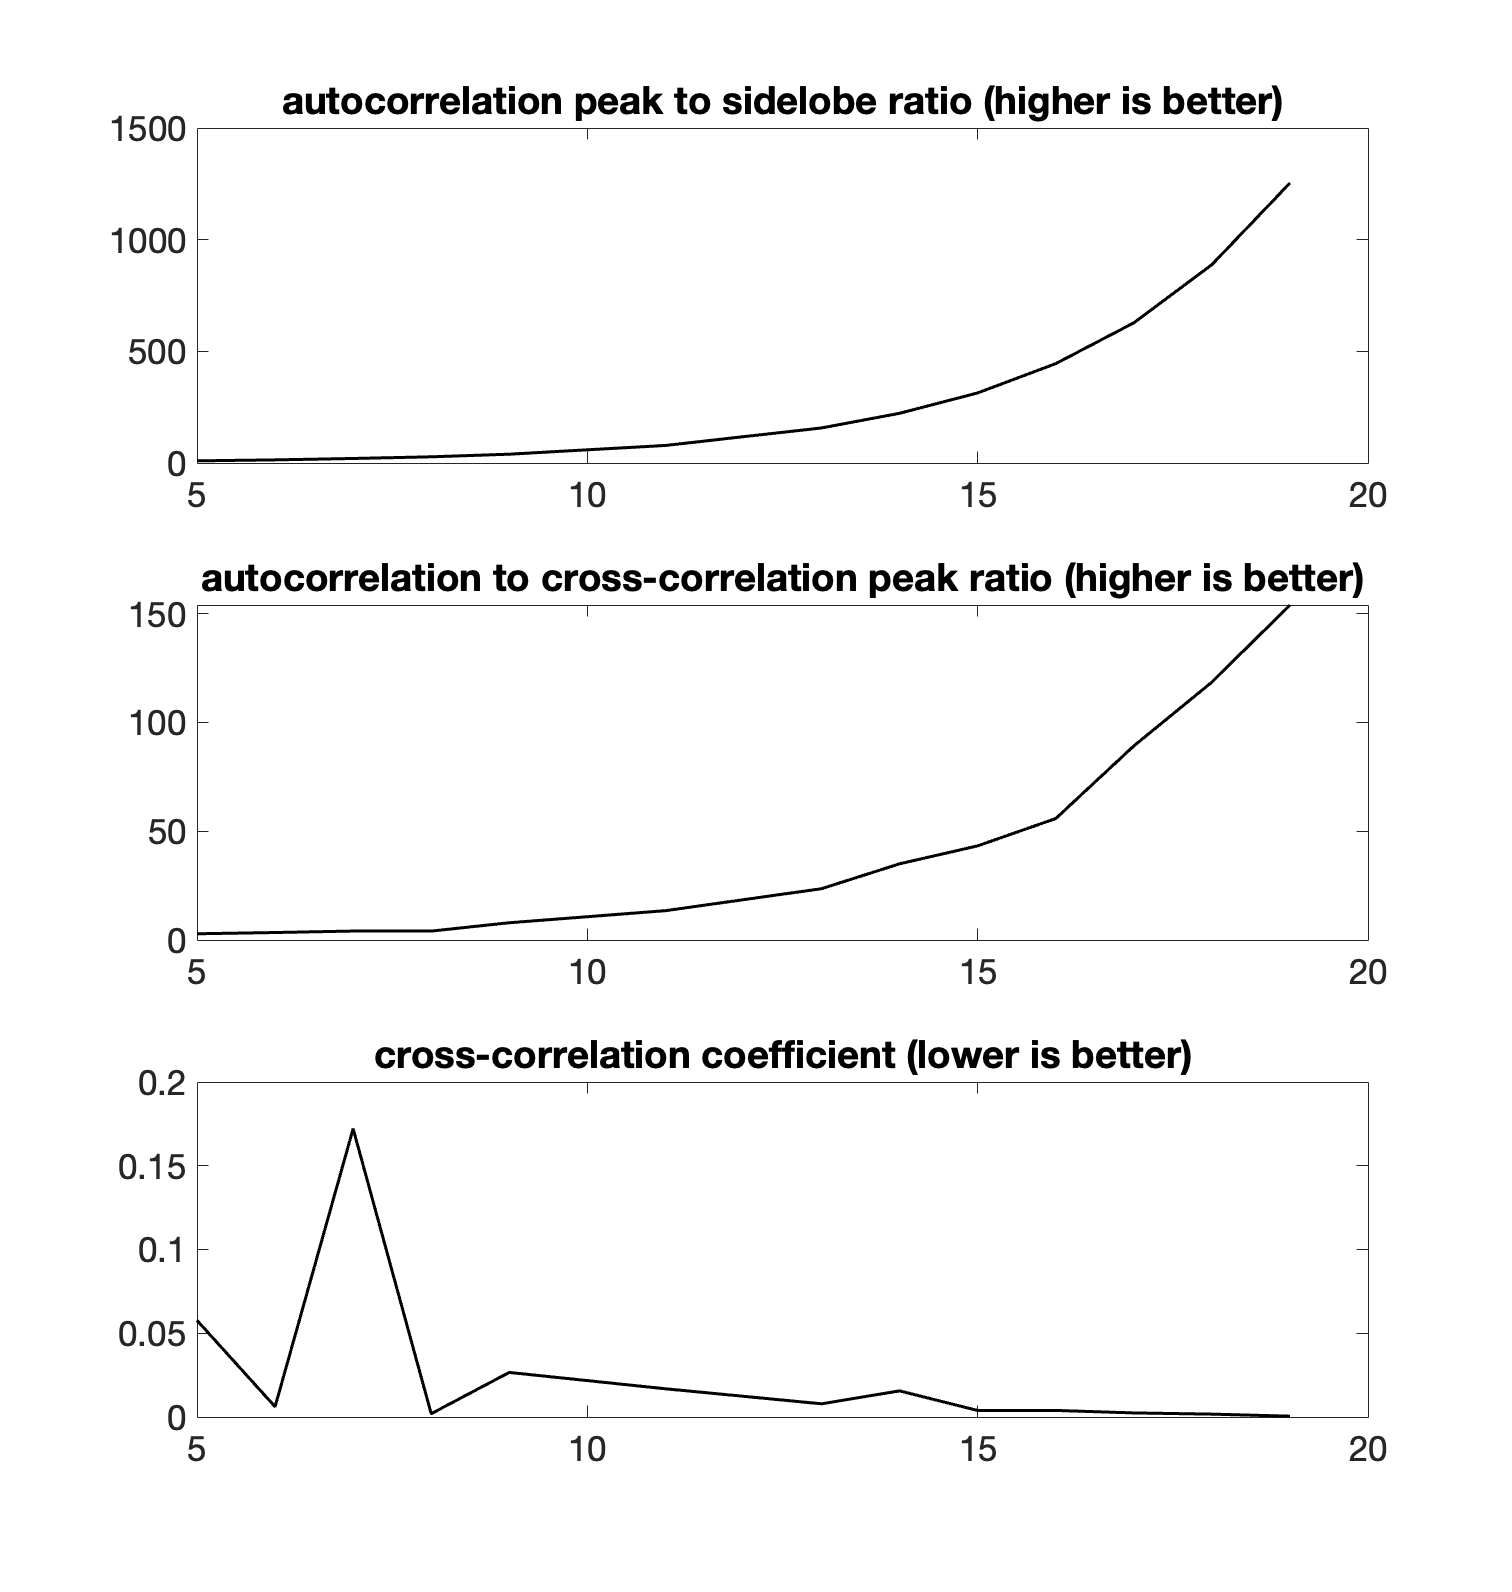
\includegraphics[width=8cm]{images/matlabplots/gold}
%
%	\caption{Gold sequence evaluation}
%\end{figure}
%
%\begin{figure}[h]
%	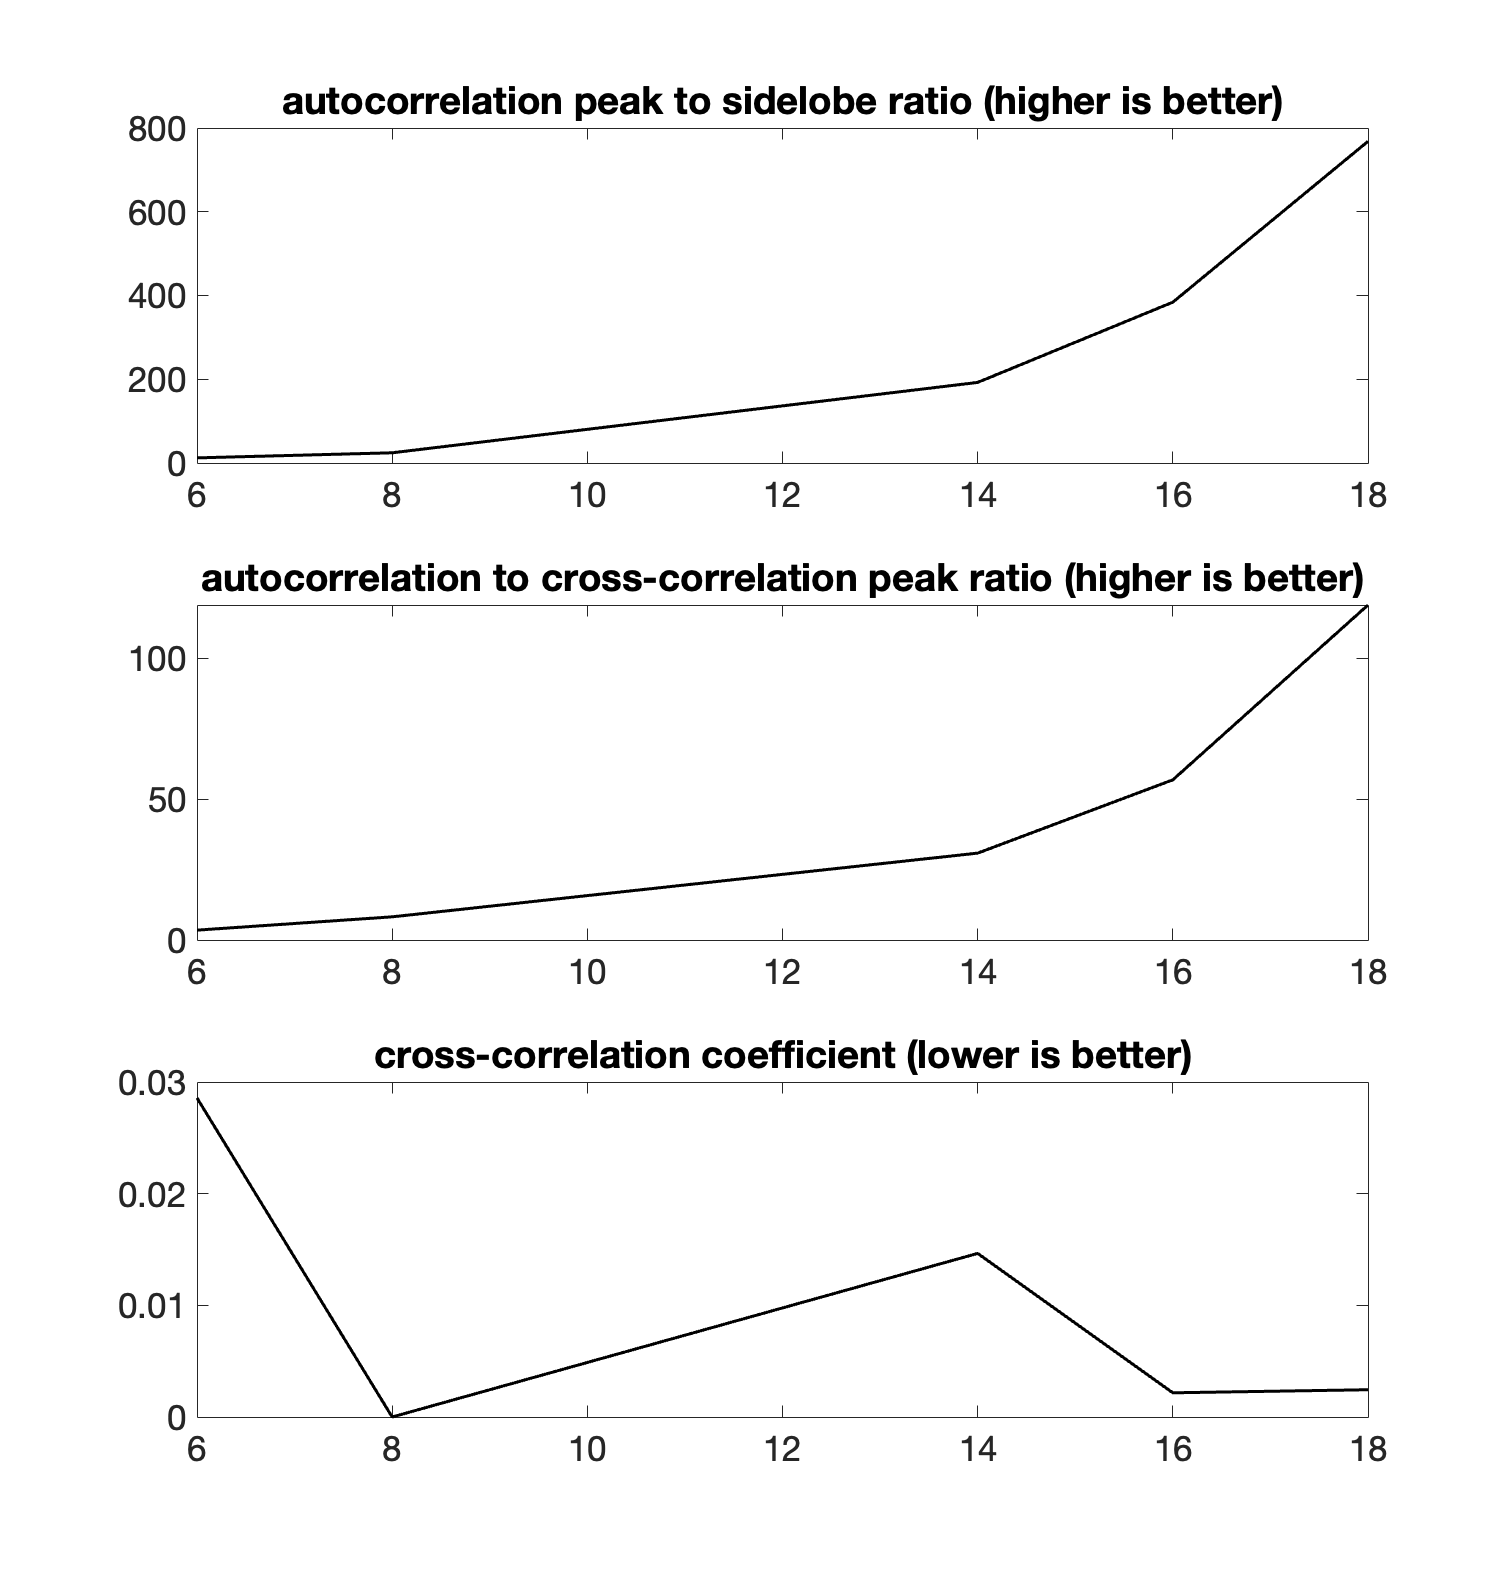
\includegraphics[width=8cm]{images/matlabplots/kasami}
%
%	\caption{Kasami sequence evaluation}
%\end{figure}
%%\fignoframe{images/matlabplots/mseq}{Basic structure of an LFSR (Linear Feedback Register). \cite{proakis08}}{fig:framelessFigures}
%%\fignoframe{images/matlabplots/gold\_10ms}{Basic structure of an LFSR (Linear Feedback Register). \cite{proakis08}}{fig:framelessFigures}
%%\fignoframe{images/matlabplots/kasami\_10ms}{Basic structure of an LFSR (Linear Feedback Register). \cite{proakis08}}{fig:framelessFigures}
%\section{Results}
In this evaluation of data, three types of codes were compared. Maximum length sequences, Gold Codes, and Kasami Codes. The performance of each code was assessed using two ratios, the ACR and the PSR.\\
From preferred polynomial all possible maximum length sequences, gold sequences and kasami sequences are generated. Then both measures are applied on the cross-correlation and auto-correlation functions of the random codes. The PSR and ACR measures are plotted against the used polynomials. Also the best case of PSR and ACR are plotted by their given correlation function.\\
Maximum length sequences hold the best auto-correlation properties in comparison to its competitors. But it shows peaks in its cross-correlation, making it a rather bad option for orthogonal separation. The kasami sequence has a way better cross-correlation but still a small peak. The clear winner are gold codes because of the good auto-correlation and very good cross-correlation properties \ref{fig:eva}. Its auto-correlations lags a bit behind its competitors but orthogonality is as much as important. 
%
%\begin{figure}[h]
%	\centering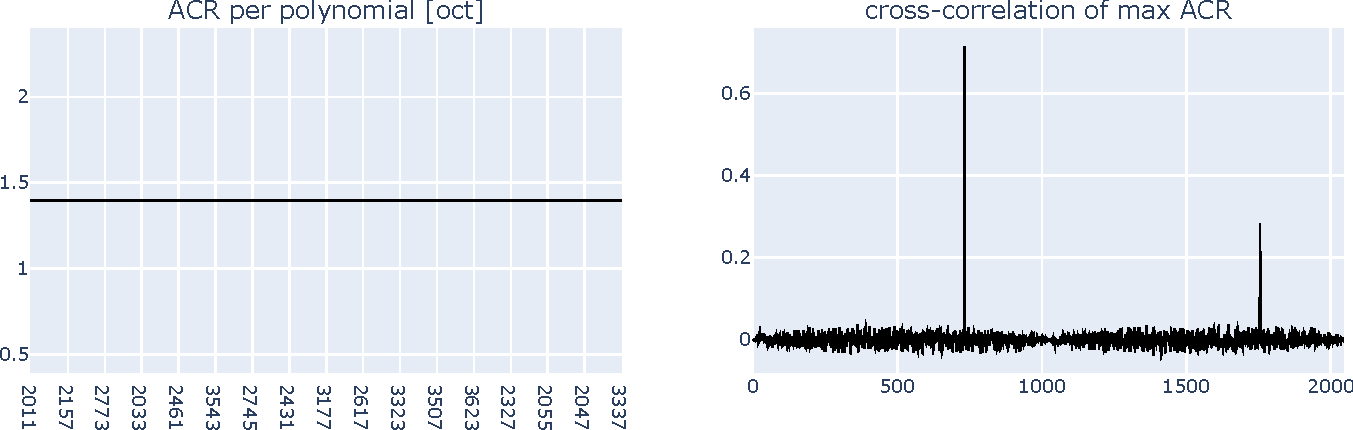
\includegraphics[width=13cm]{images/mseqevaacr}
%	
%	\caption{Evaluation of m-sequences by AC ratio}
%	\label{fig:eva}
%\end{figure}
%
%\begin{figure}[h]
%	\centering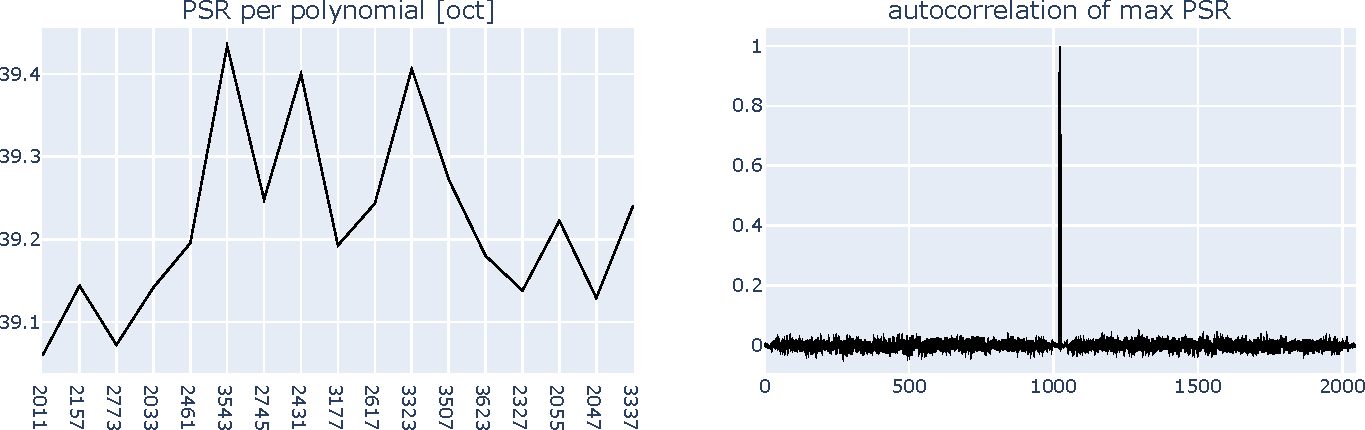
\includegraphics[width=13cm]{images/mseqevapsr}
%	
%	\caption{Evaluation of m-sequences by PS ratio}
%	\label{fig:eva}
%\end{figure}

\begin{figure}[h]
	\centering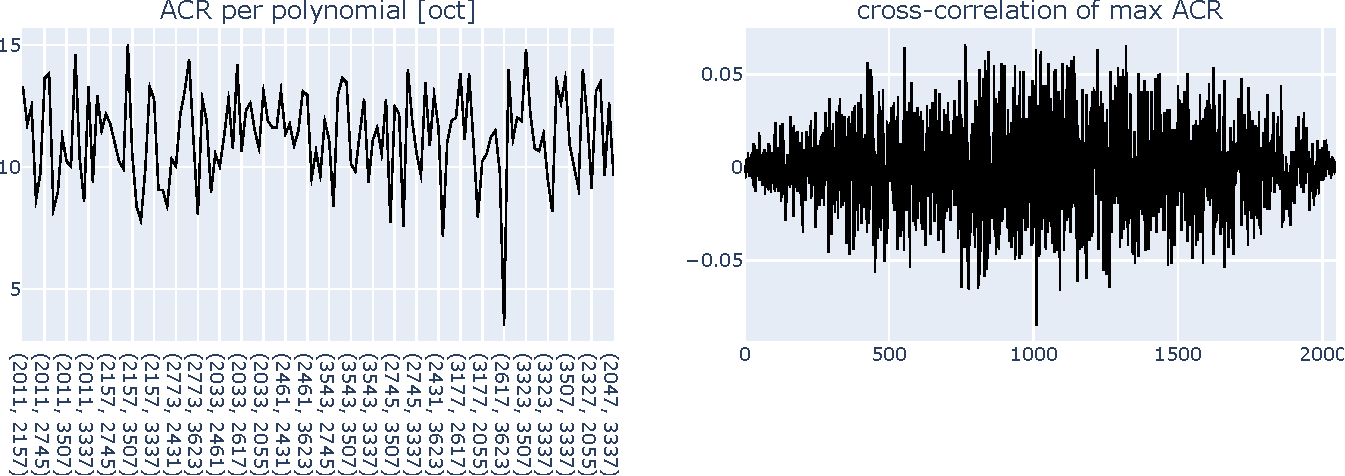
\includegraphics[width=14cm]{images/goldevaacr}
	
	\caption{Evaluation of gold sequences by AC ratio}
	\label{fig:eva}
\end{figure}

\begin{figure}[h]
	\centering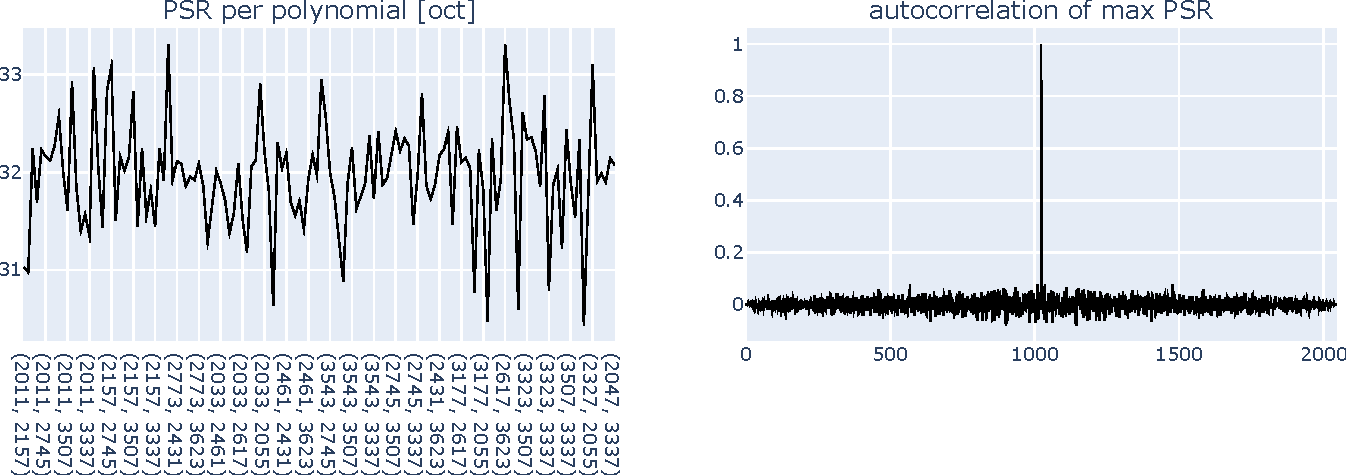
\includegraphics[width=14cm]{images/goldevapsr}
	\caption{Evaluation of gold sequences by PS ratio}
	\label{fig:eva}
\end{figure}
To get more valuable data, elements from each set of codes are sampled uniformly ($N=1000$) and afterwards the evaluation parameters are applied.
The results yields that Gold Codes had the least increase in PSR, but were the second best at ACR. Kasami Codes were only slightly better in both PSR and ACR than Gold Codes, but had a smaller set of codes available. Maximum length sequences had the highest PSR, but the worst ACR.\\
Based on these findings, it can be concluded that Gold Codes are the best choice for this application. While maximum length sequences had the highest PSR, they performed poorly in terms of ACR. Gold Codes, on the other hand, had a good balance of performance in both ratios, and also had a large set of codes available. In addition, Gold Codes demonstrated better cross-correlated detection compared to maximum length sequences.
\begin{figure}[h]
	\centering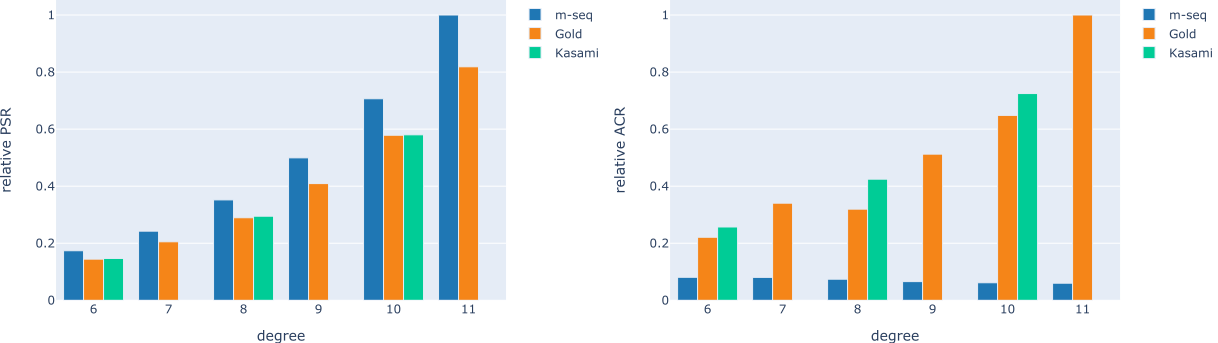
\includegraphics[width=14cm]{images/degCompEva}
	
	\caption{Evaluation by relative PSR for degrees 6 to 11}
	\label{fig:eva}
\end{figure}

%\begin{figure}[h]
%	\centering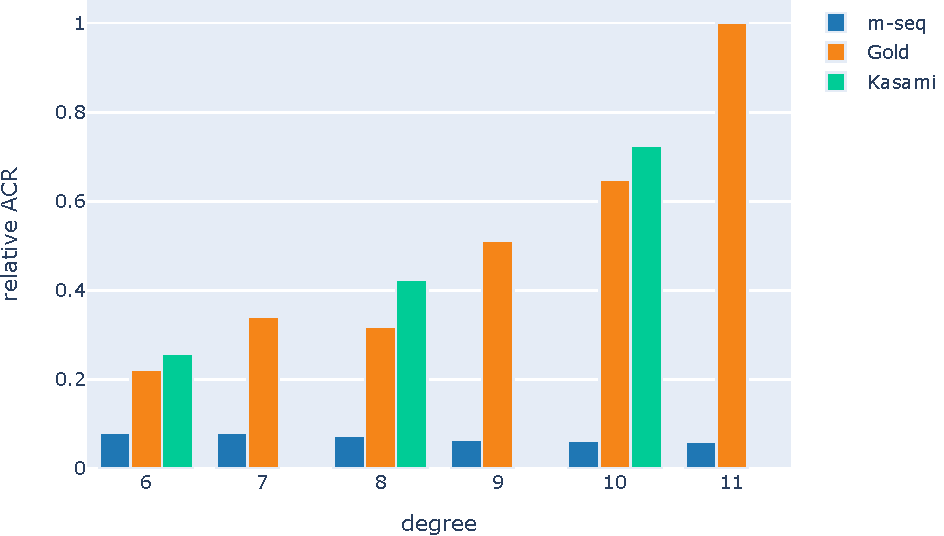
\includegraphics[width=13cm]{images/degAcrEva}
%	
%	\caption{Evaluation by relative ACR for degrees 6 to 11}
%	\label{fig:eva}
%\end{figure}


\chapter{Signal Processing}
The signal processing is separated into two sections. First the code needs to be transformed into the base-band. After that a spectrum shift to a specific transmission band is realized. Afterwards the exported signal is put through an simulator which adds reflection noise. The result is than again imported and gets reverse spectrum shifted. At the end a peak detection method is used to ignore reflection peaks.
\section{Base-Band}
Before a spectrum shift is applied to the signal, the bandwidth needs to be bounded. Otherwise absolute code bits would result in theoretically infinite frequencies which are impossible to implement for transmission. A raised cosine filter is therefore applied to remove all unwanted frequencies above a certain threshold. The base-band for our application is $20kHz$. Thus, our symbol length is set to $1/{20kHz}$. A appropriate roll-off coefficient of $0.125$ is picked. The resolution of cosine needs to be high enough to include at least a couple of periods.  A whole cosine is not tangible because its periodic and therefore infinite in time.
\begin{figure}[h]
	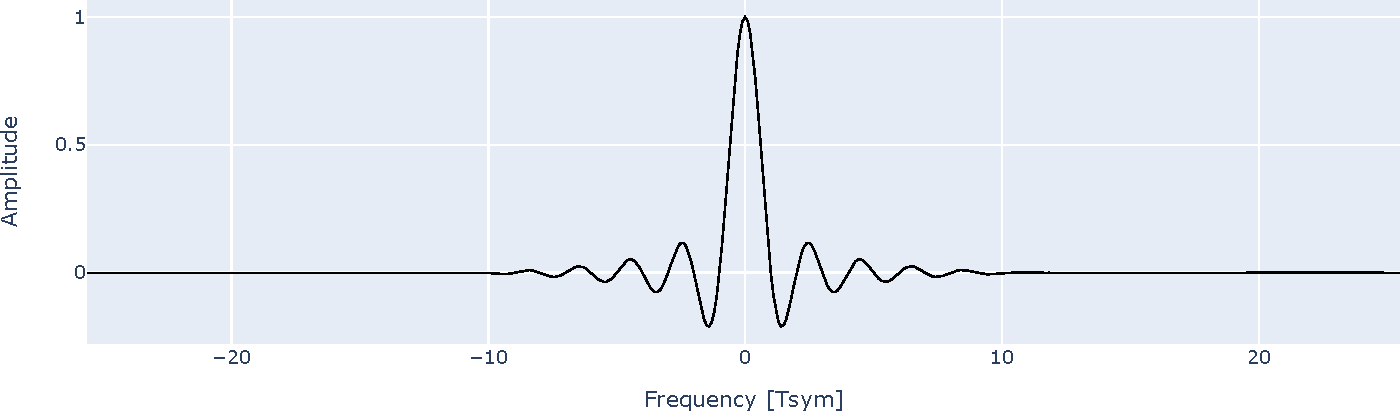
\includegraphics[width=\linewidth]{images/cosfir}
	\caption{Section of Cosine FIR with a resolution of 1024}
	\label{fig:cosfir}
\end{figure}
\section{Transmission ans Base-Band Shifting}
Now the spectrum is ready to be shifted by the given transmission frequency $f_c$. The resulting signal could hold imaginary parts, hence we only move the real part further in processing. The inverse shift works by applying the negative transmission frequency.
\begin{equation}
	x_{TB}[k]=Re\{x_{BB}[k]\cdot e^{-2\pi j f_c k}\}
	\label{eq:shift}
\end{equation}
\begin{equation}
	x_{BB}[k]=x_{TB}[k]\cdot e^{-2\pi j (-f_c) k}
	\label{eq:rshift}
\end{equation}

\section{Simulation}
The simulation consists of a watermark benchmark \cite{watermark15} and a additive GWN generated by a desired SNR between $-20dB$ and $20dB$ in steps of $5dB$. From the general equation of the Signal to Noise Ratio we derive our noise standard deviation by transforming this ratio. The white noise is added after the simulation and before receiver filtering.
\begin{equation}
	SNR=\cfrac{P_{Signal}}{P_{Noise}}=\cfrac{\mathbb{E}({Signal}^2)}{\mathbb{E}({Noise}^2)}=\cfrac{\sum {Signal}^2}{N\cdot\sigma_{Noise}^2}~~\Leftrightarrow~~\sigma_{Noise}=\sqrt{\cfrac{\sum^N {Signal}^2}{N\cdot SNR}}
\end{equation}

\begin{equation}
	SNR_{dB}=10\cdot\log_{10}\cfrac{\sum Signal^2}{\sum Noise^2}=10\cdot\log_{10}\cfrac{\sum^N_{k=1} x_{TB}^2[k]}{\sum^N_{k=1} Noise^2[k]}
\end{equation}

\begin{equation}
	Noise=\text{\textsc{Normal}}(0,1)\cdot \cfrac{\sigma_{Signal}}{SNR}
\end{equation}


\section{Low-pass Filter}

A flat magnitude is favorable because only frequencies of the base-band should be passed through. Such a filter, namely a maximally flat magnitude or Butterworth filter, approximates this goal. The roll-off decreases by increasing the order of the system.\\
The filter gets applied after shifting back to the base-band. The spectrum shift works almost the same as the first one \ref{eq:shift}, but with an sign change in the exponent. Most noise and reflections get reduced if their frequencies do not reach the base-band.
\begin{figure}[h]
	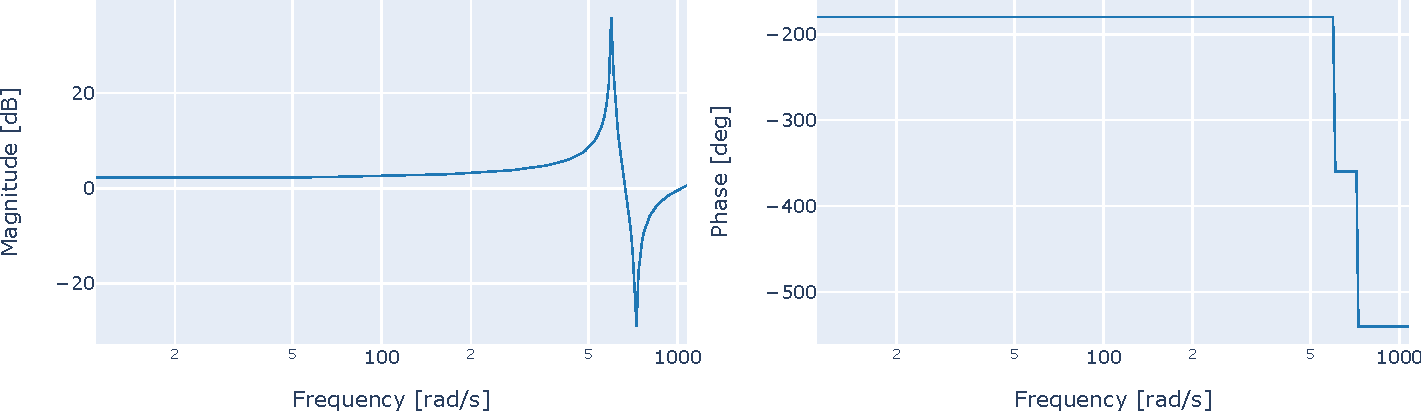
\includegraphics[width=\linewidth]{images/bode}
	
	\caption{Bode plot of 5th order Butterworth low-pass filter}
	\label{fig:bode}
\end{figure}

\section{Peak detection}
The received signal, consisting of summed delayed signals, cross-correlated by every anchor. If the signal is not reflected the peak in cross-correlation would be obvious. But because by the introduction of noise and water reflections a higher rate of similar peaks appear. To suppress these effects a CA-FAR Algorithm \cite{rohling11} is applied to only detect the first reflected peak resulting in lower false alarms of peaks. \\
CA-FAR works by using multiple values intervals. The most outer one could be described as a train bin and is used to get an estimation of the signals noise. Especially CA-FAR uses averaging to estimate the noise by measured cells. The bordering bin, defined as the guard cells, is used to reduce self-interference of the peaks. Thus, increasing window sizes $N$ resulting in better noise estimating but still limited by the sample rate \ref{eq:cft} \cite{rohling11}\cite{radarbasics}. By knowledge of measured peak widths a optimal guard interval can be figured.\\
The calculated threshold is than scaled by a formula depending on the false alarm rate. The higher the false alarm rate, the weaker high amplitude peaks gets included by the threshold \ref{eq:cff}.\\
Because Cell Averaging shows not satisfactory results in sensitive multi targets examples, the noise estimation could be enhanced by a sorting average. That principle is defined as CO-FAR \cite{rohling11}. 
\begin{center}
	\begin{tabular}{|c|c|}
		\hline
		candidate sample & $i$\\
		\hline
		guard interval (half) & $\mathcal{G}$ \\
		\hline
		train interval (half) & $\mathcal{T}$ \\
		\hline
		false alarm rate & $\eta$\\
		\hline
	\end{tabular}
	\linebreak
\end{center}

\begin{equation}
	Threshold(i)_x=
	\cfrac{\alpha}{2\mathcal{T}}
	\left[ \sum_{j=i-\left( \mathcal{G}+\mathcal{T}\right) }^{i+\left( \mathcal{G}+\mathcal{T}\right)}x(j) - \sum_{j=i-\mathcal{G}}^{i+\mathcal{G}}x(j) \right] 
	\label{eq:cft}
\end{equation}
\begin{equation}
	\text{scale factor}~~~
	\alpha=2\mathcal{T}\left( \eta^{-1/{2\mathcal{T}}}-1\right) 
	\label{eq:cff}
\end{equation}
%\chapter{Implementation in Python}

For the Implementation python 3.10 is used. The signal generation and processing is based on the use of the libraries compy, scipy and numpy. Graphical plotting is realized by the use of the plotly library, which generates plots as a interactive html file. 

\section{Documentation - Signal Processing}




\chapter{Evaluation}
This evaluation outlines the process of testing the performance of the localization system using orthogonal codes in underwater environments. The chapter covers the simulation of the system, in which a benchmark is used to assess the performance with different levels of SNR by adding white noise. 

Additionally, the chapter discusses the field testing of the algorithm, which is performed in a real-world scenario using three hydrophones configured as two sending anchors and one receiver. The simulation and field testing results provide valuable insights into the accuracy and reliability of the localization system.
\section{Simulation}
The simulation part involves the use of a Watermark benchmark \cite{watermark15} and the addition of Gaussian white noise with varying levels of signal-to-noise ratio (SNR) to the signals. The simulation then evaluates the performance by following a simulated path of positions in 3D space, using four anchors.
\subsection{Watermark}
The Watermark Simulation consists of a convolution or channel replay by an selected channel TVIR estimate. The channels consist of multiple dirac impulses of different strengths. Thus, reflections and reduced signal strength are simulated.\
\begin{equation}
	x_{tSigTBr}[k]=\sum_{i=0}^{N}h[k,i]\cdot x_{tSigTB}[k-i]
\end{equation}

\subsection{White noise}
A additive Gaussian White Noise (GWN) generated by a desired Signal to Noise Ratio (SNR) between \SI{-20}{\decibel} and \SI{20}{\decibel} in steps of \SI{5}{\decibel}. From the general equation of the Signal to Noise Ratio we derive our noise standard deviation by transforming this ratio. The white noise is added after the simulation and before receiver filtering. To estimate the power of our signal a standard deviation estimation is used, which consists of all incoming signals by using its expected value. The Gaussian noise is generated by using a normal distributed random variable with its mean at zero and its standard deviation at $\frac{\bar{\sigma}}{SNR}$. Thus, $M$ denotes the number of total anchors and $N$ is the length of the corresponding signal.
\begin{equation}	
	\bar{\sigma}=\cfrac{1}{M}\sum_{i=0}^{M}\sigma_i,~~~\sigma_j=\sum_{k=0}^{N}{tSigTBr_j}^2[k]
\end{equation}
\begin{equation}
	n[k]=f_{GWN}[k]\cdot \cfrac{\bar{\sigma}}{SNR},~~~GWN\sim\text{Normal}(0,1)
\end{equation}
\begin{figure}[h]
	\centering
	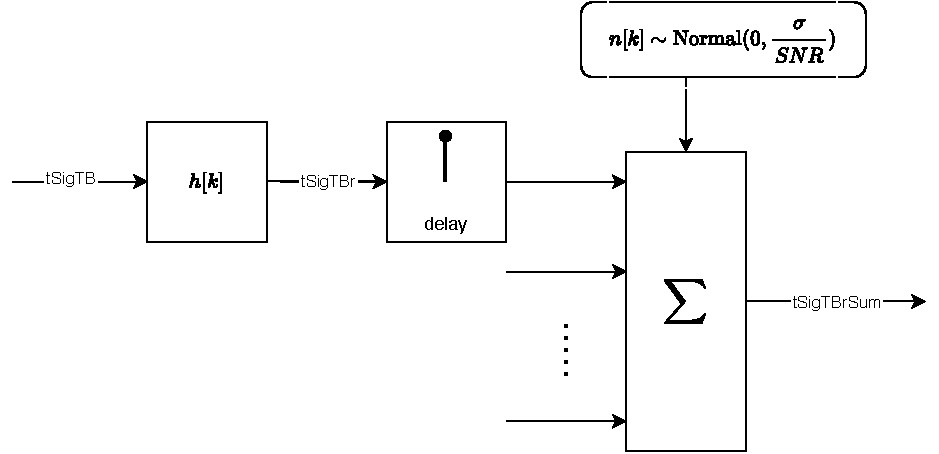
\includegraphics[width=\linewidth]{images/simsig}
	
	\caption{Simulation of acoustic signal underwater propagation}
	\label{fig:simsig}
\end{figure}

\subsection{Localization simulation}
To test the localization algorithm, several 3-dimensional space paths were simulated, wherein the generated points formed a helical curve that expanded in the $z$-direction \ref{eq:helix}. The positions of four anchors were utilized to calculate the TDOA values using multilateration techniques, which were subsequently incorporated into the localization algorithm \ref{eq:dist2toa}. Further, an approximate value of \SI{1500}{\meter\per\second} for the speed of sound $c$ in water was used as a parameter in the calculations. Multiple runs, utilizing varying SNR's and watermark channels were conducted to evaluate the performance of the peak detection method.

\begin{equation}
	\vec{x}_{\phi}(\alpha,\beta)
	=\left[
	\begin{array}{c}
		\alpha\cdot\sin{\phi}+\beta\\
		\alpha\cdot\cos{\phi}+\beta\\
		-|\phi| \leq z \leq -1
	\end{array}
	\right]
	\label{eq:helix}
\end{equation}
\begin{equation}
	\tau_i = \frac{1}{c} \cdot \left(\left| S - S_0 \right | - \left | S - S_i \right|\right)
	\label{eq:dist2toa}
\end{equation}
The simulation system is based on 20 simulated positions. An almost rectangle coverage for the target is created using four anchor coordinates $S_0=(\SI{15}{\meter},\SI{1}{\meter},\SI{17}{\meter})$, $S_1=(\SI{200}{\meter},\SI{10}{\meter},\SI{5}{\meter})$, $S_2=(\SI{195}{\meter},\SI{210}{\meter},\SI{6}{\meter})$ and $S_3=(\SI{16}{\meter},\SI{190}{\meter},\SI{3}{\meter})$ to be located in. The circular curve is scaled by \SI{30}{\meter} and has an offset of \SI{100}{\meter} from the point of origin.  The CA-FAR lower threshold is set to $0.2$ to exclude accidental peak detection in low amplitude correlation phases.

The results of the simulation of position detection indicate that, as the noise level increases and the signal-to-noise ratio decreases, some positions cannot be accurately located \ref{fig:3dvs1}. This intrusion of noise leads to a failure of the peak detection due to new peaks with high similarity to the real ones. The correlations reveal that, with increased noise, the side lobes of the correlation peaks become more prominent, making it difficult to detect peaks \ref{fig:3dvslines1}. Additionally, a higher CFAR threshold, which is a side effect of the additive noise, may result in the rejection of valid peaks.

\begin{figure}
	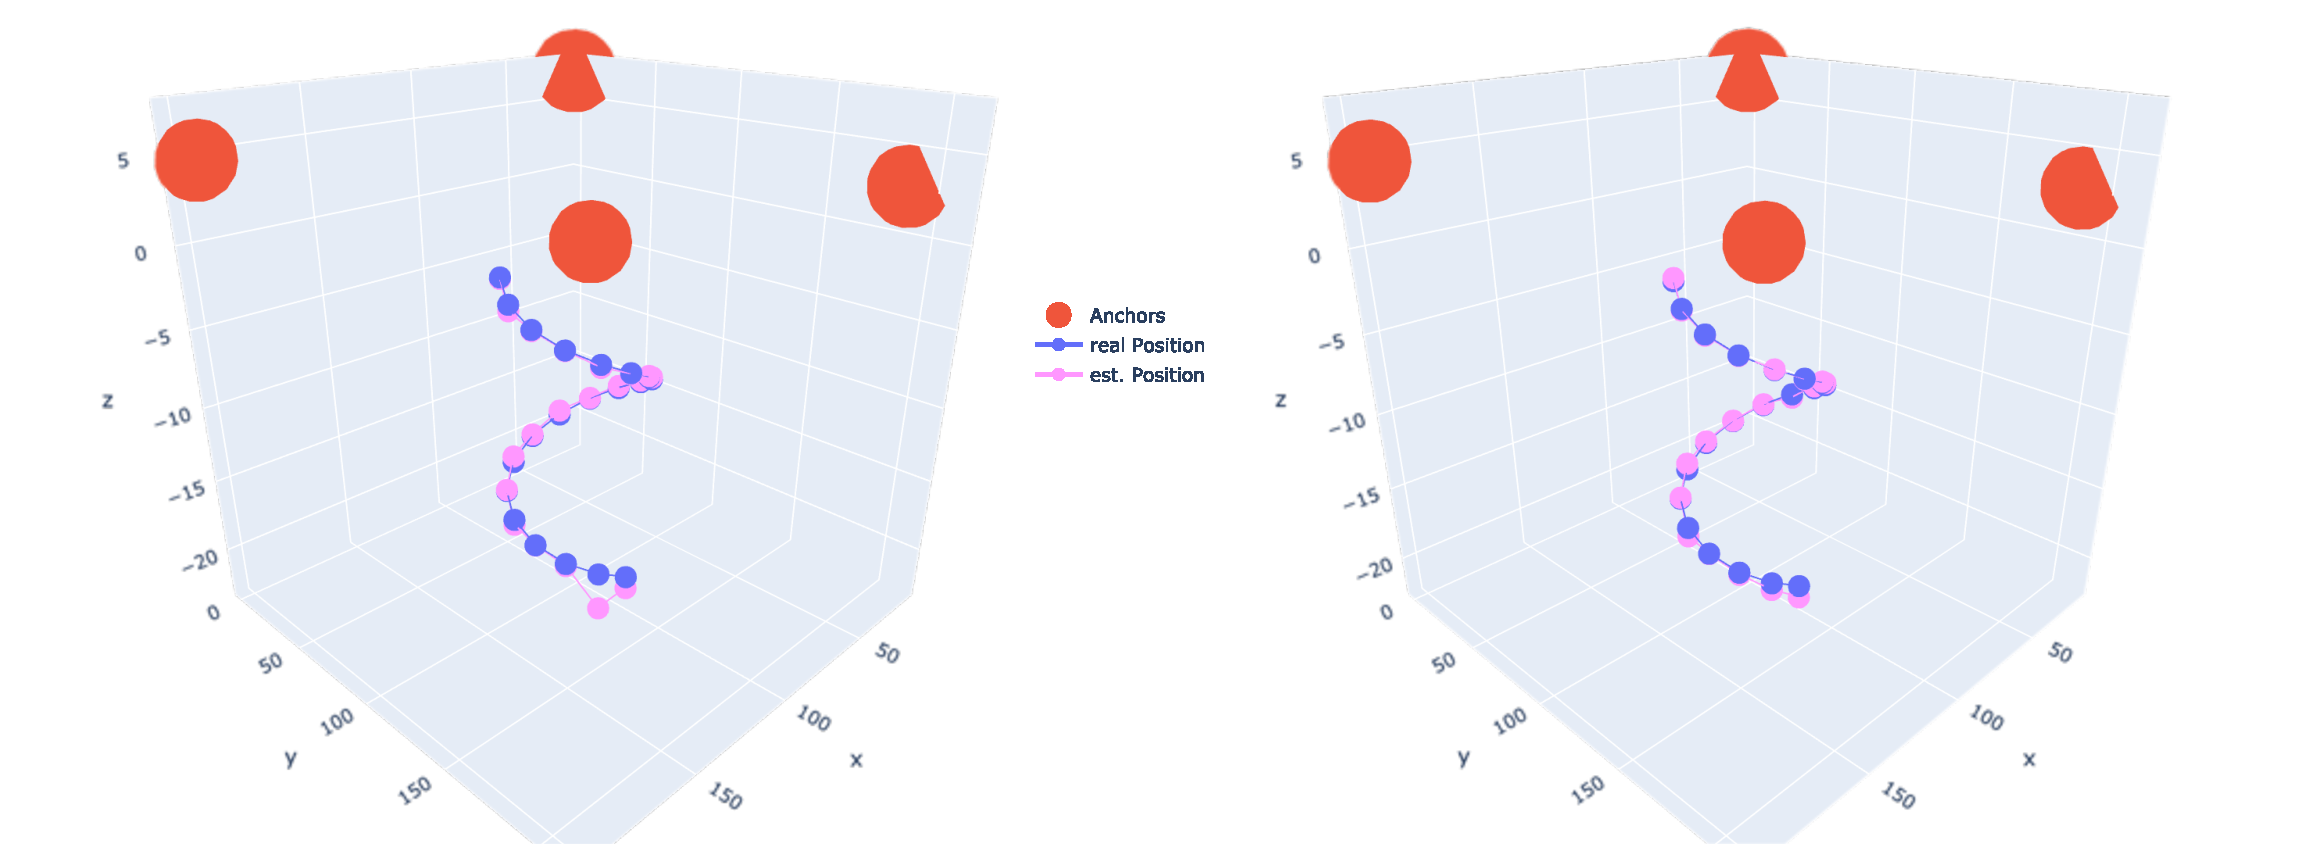
\includegraphics[width=\linewidth]{images/simulation/d10-5snrvs20snr} 
	\caption{3D position evaluation with code of 10th degree. Left one shows \SI{-5}{\decibel} and right one \SI{20}{\decibel} signal strength created by additive noise.}
	\label{fig:3dvs1}
\end{figure}
\begin{figure}
	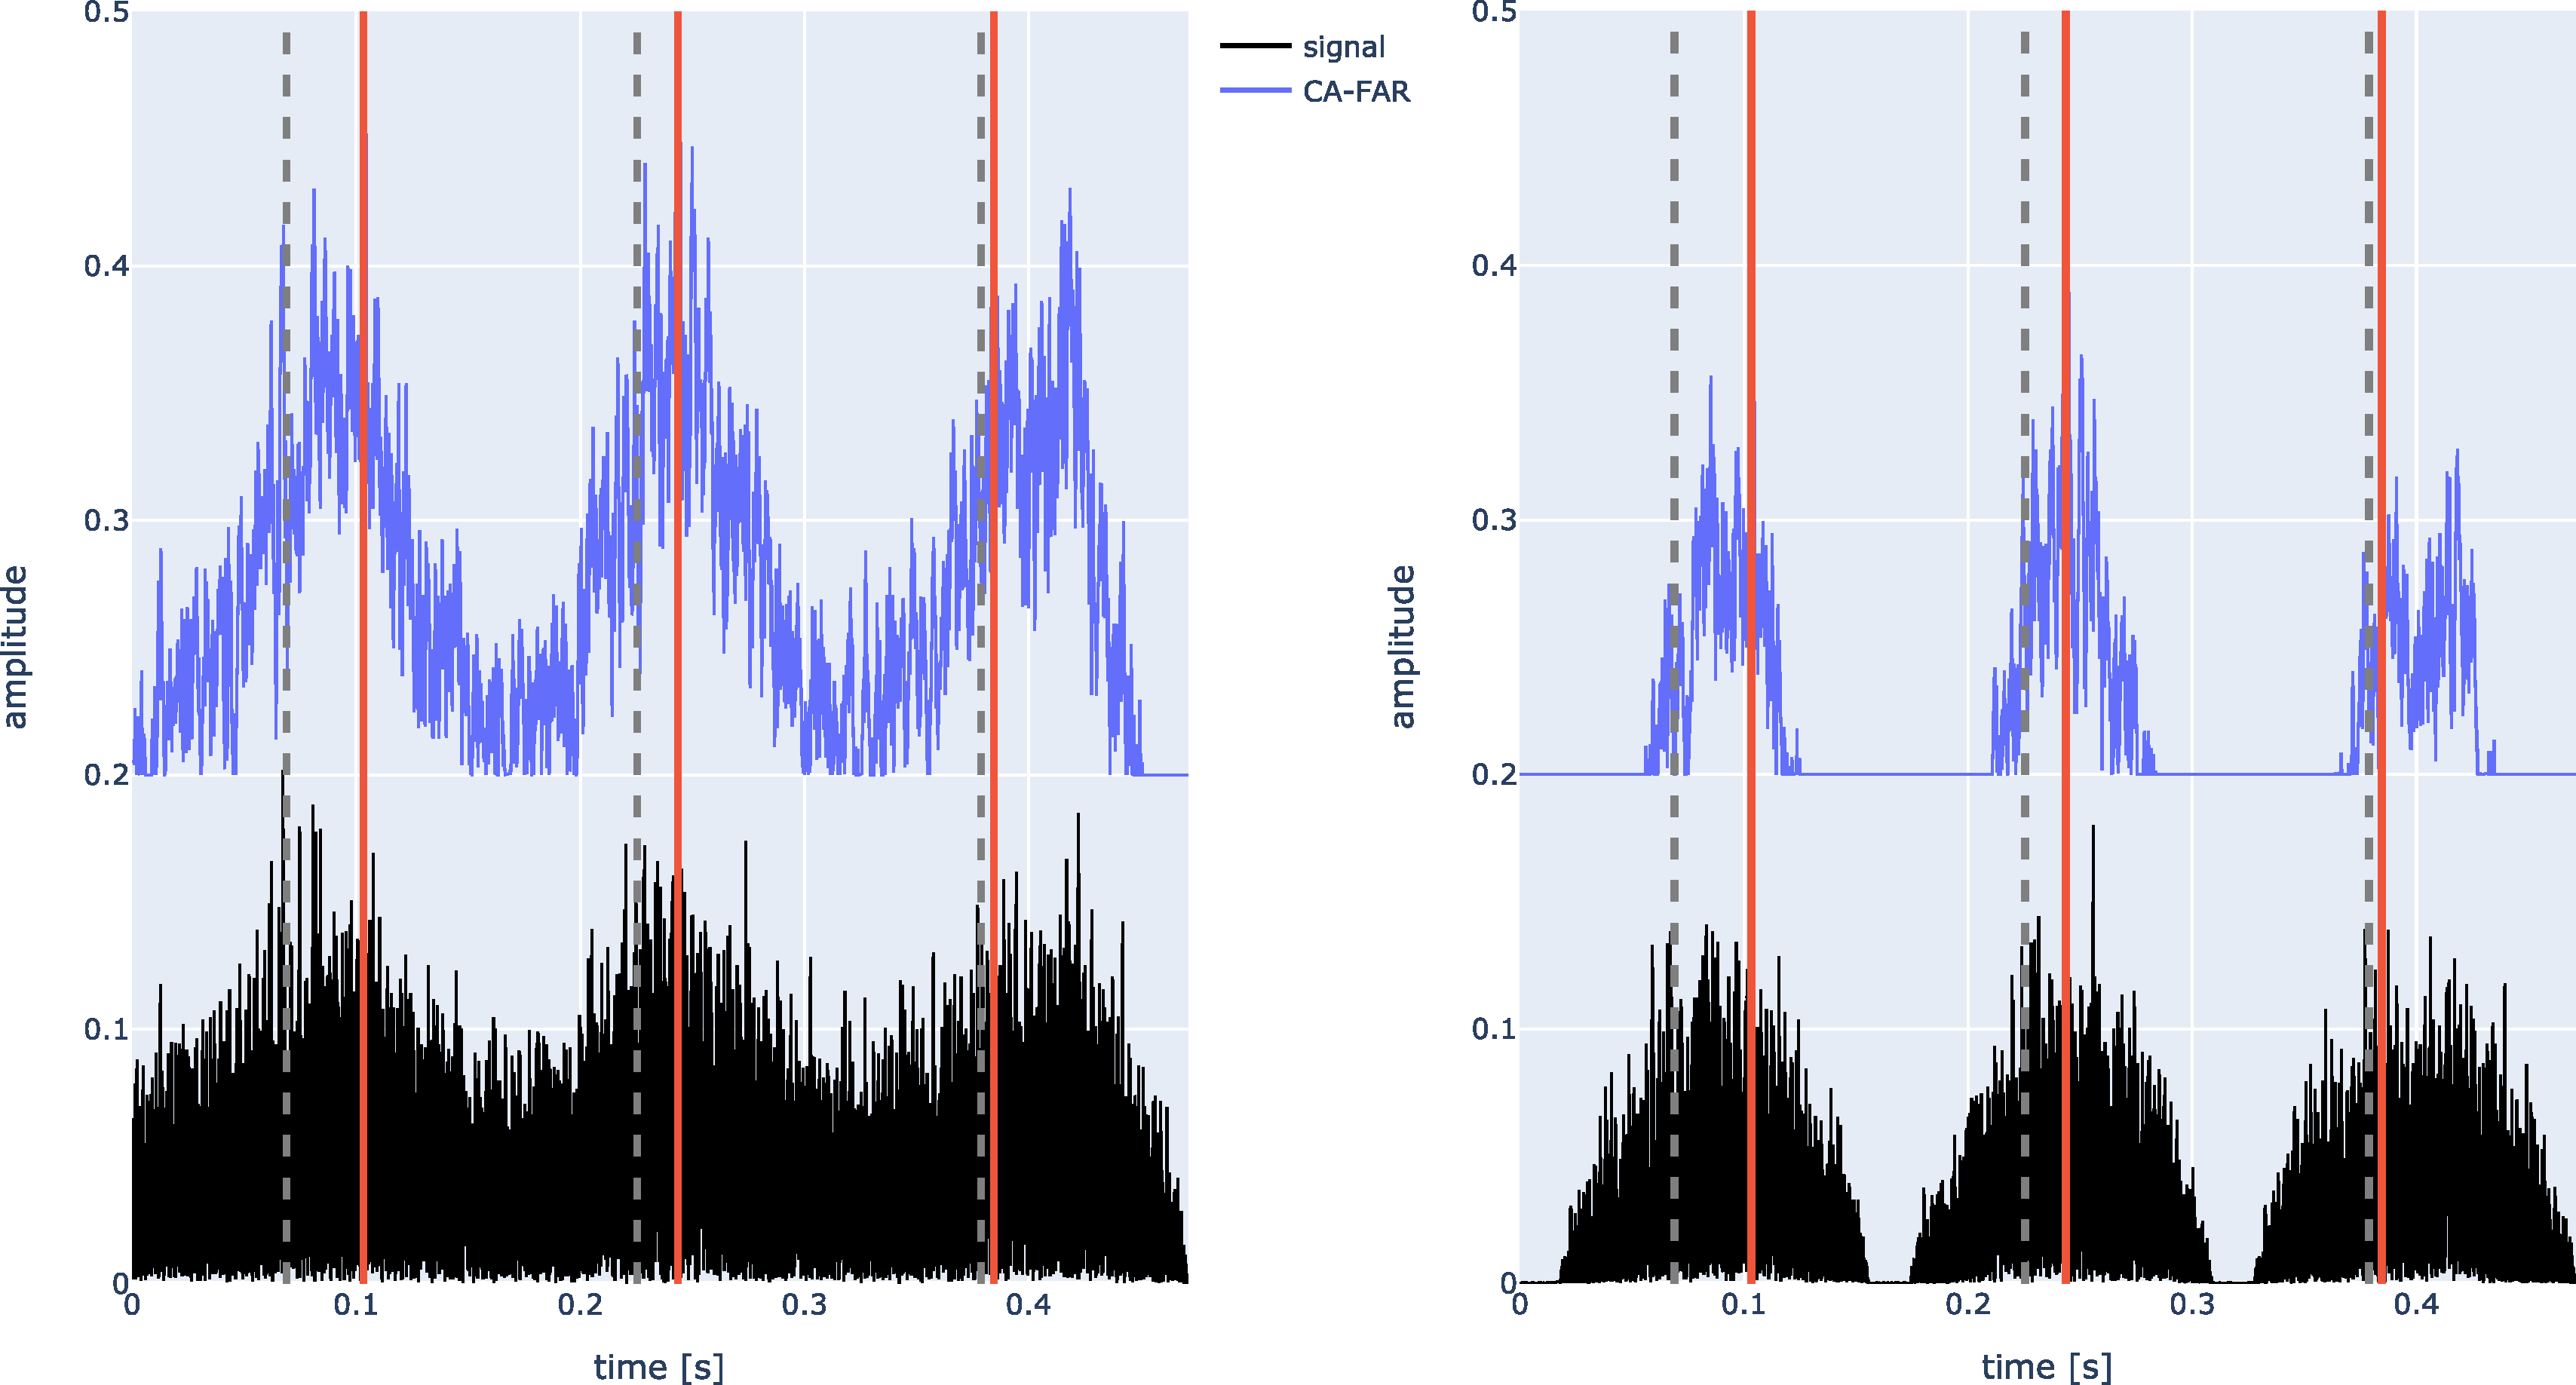
\includegraphics[width=\linewidth]{images/simulation/d10snr-5vs20lines} 
	\caption{Correlation of an anchor for first three positions. The gray dotted line marks the first peak of the period, the red line one of the current correlating anchor.}
	\label{fig:3dvslines1}
\end{figure}
By iterating though SNR's between \SI{-5}{\decibel} and \SI{20}{\decibel} in steps of \SI{1}{\decibel} shows that the mean error, which is the average absolute difference between the calculated and expected positions, increases when the SNR is less than \SI{8}{\decibel} and jumps to even higher levels due to the increasing likelihood of false peak detection \ref{fig:errorsnr}.
\begin{figure}
	\centering
	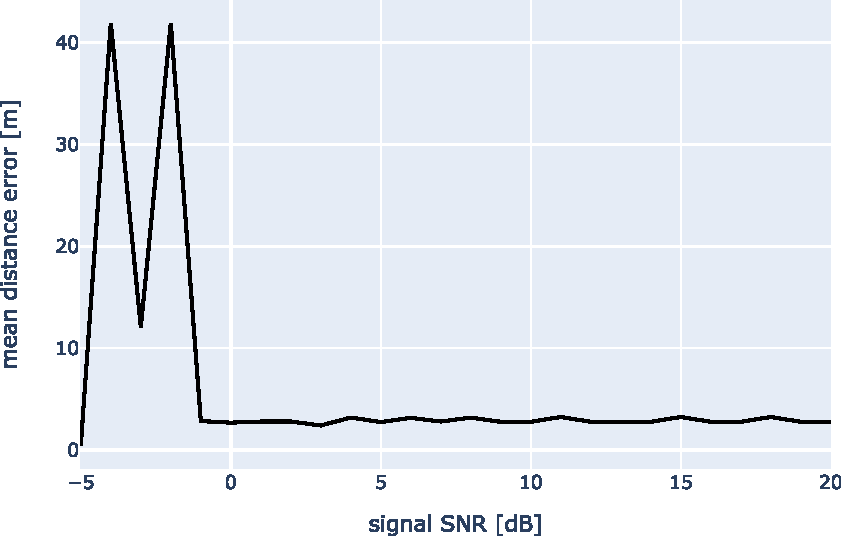
\includegraphics[width=8cm]{images/simulation/snrerror1} 
	\caption{Relationship between SNR and mean distance error}
	\label{fig:errorsnr}
\end{figure}
Continuing with the use of the \SI{-5}{\decibel} SNR the position detection system now incorporates watermark simulations as well. Due to multipath propagation caused by reflections from surfaces, the correlation amplitudes become even higher than those from additive noise \ref{fig:3dvslines2}. As a result, peak detection becomes less reliable, and it becomes necessary to adjust the false alarm rate.
\begin{figure}
	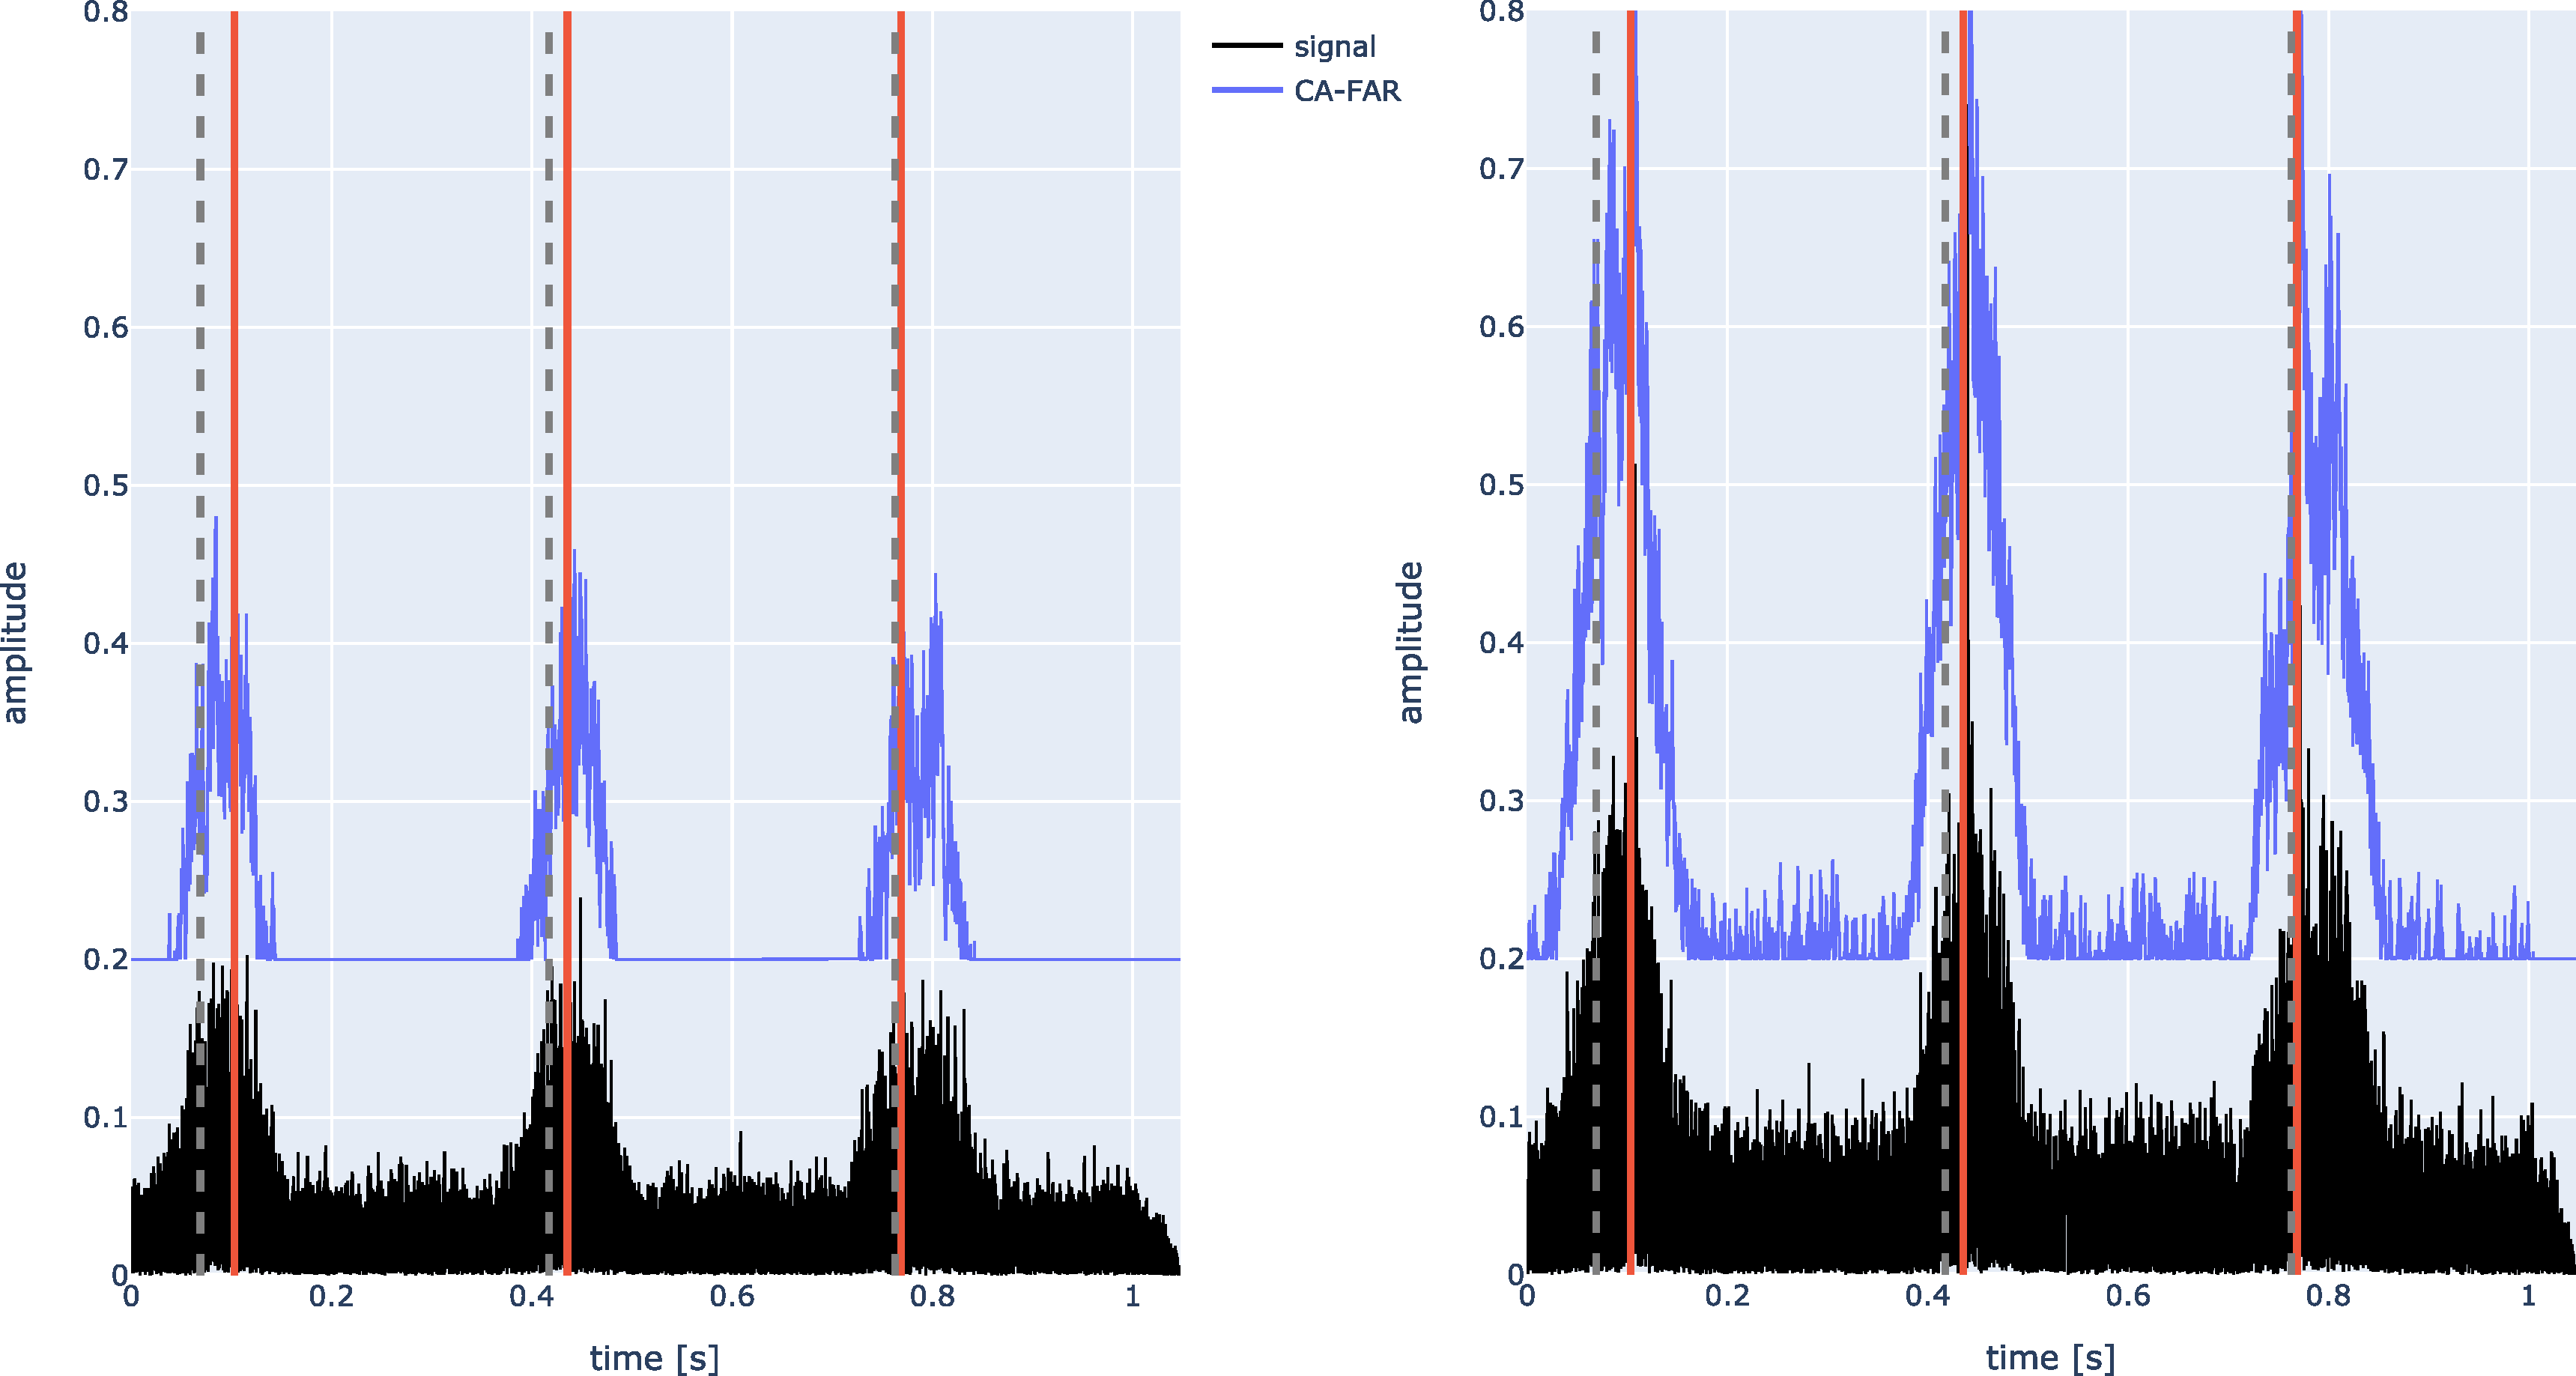
\includegraphics[width=\linewidth]{images/simulation/d10plane1vscastle2lines} 
	\caption{Correlation of an anchor for first three positions using watermark simulation channel PLANE1 at the right and CASTLE2 at the left, both with additive white noise of \SI{-5}{\decibel}}
	\label{fig:3dvslines2}
\end{figure}
\newpage
\section{Localization field testing}
A field test was conducted at a shoreline location. Three hydrophones were deployed at a depth of one meter below sea level. Anchors A and B were positioned with a distance of \SI{4.1}{\meter} between them, with Anchor B located \SI{10.74}{\meter} from the receiving hydrophone. During the test, the underwater speed of sound, as measured using a CTD Sensor (Conductivity, Temperature, and Depth), was \SI{1430.3}{\meter\per\second}. The receiving hydrophone was also relocated to a second location, \SI{5.56}{\meter} from Anchor B.

In the first run codes of degree ten were transmitted for a total time of \SI{50}{\second}. Afterwards the receiving hydrophone was moved \SI{5.18}{\meter} further away from the anchors. Then again three test runs were done with code degrees of ten, nine and seven. Every run was repeated with a more decreased signal intensity for testing lower SNR's.
\begin{figure}
	\centering
	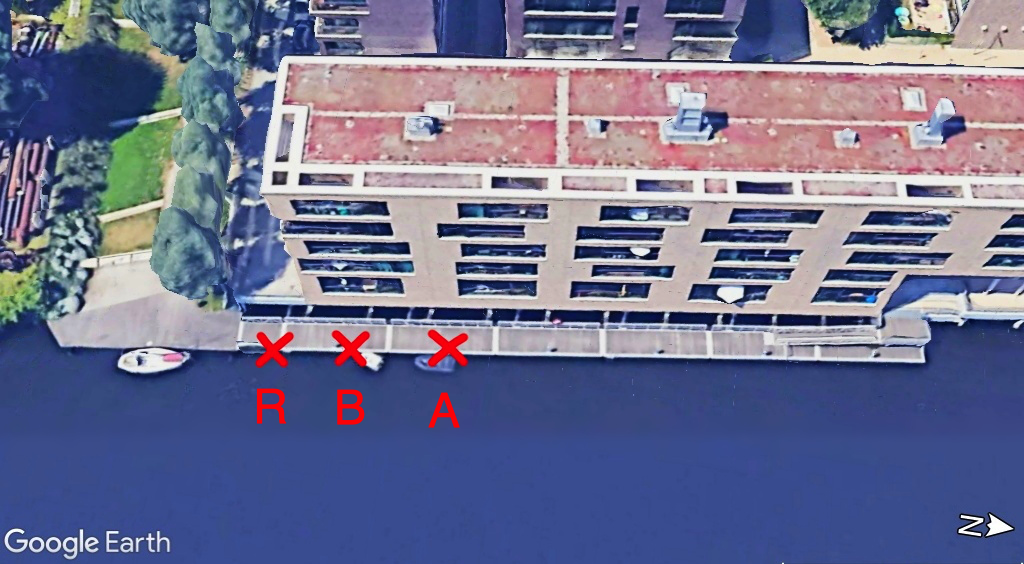
\includegraphics[width=12cm]{images/labloc}
	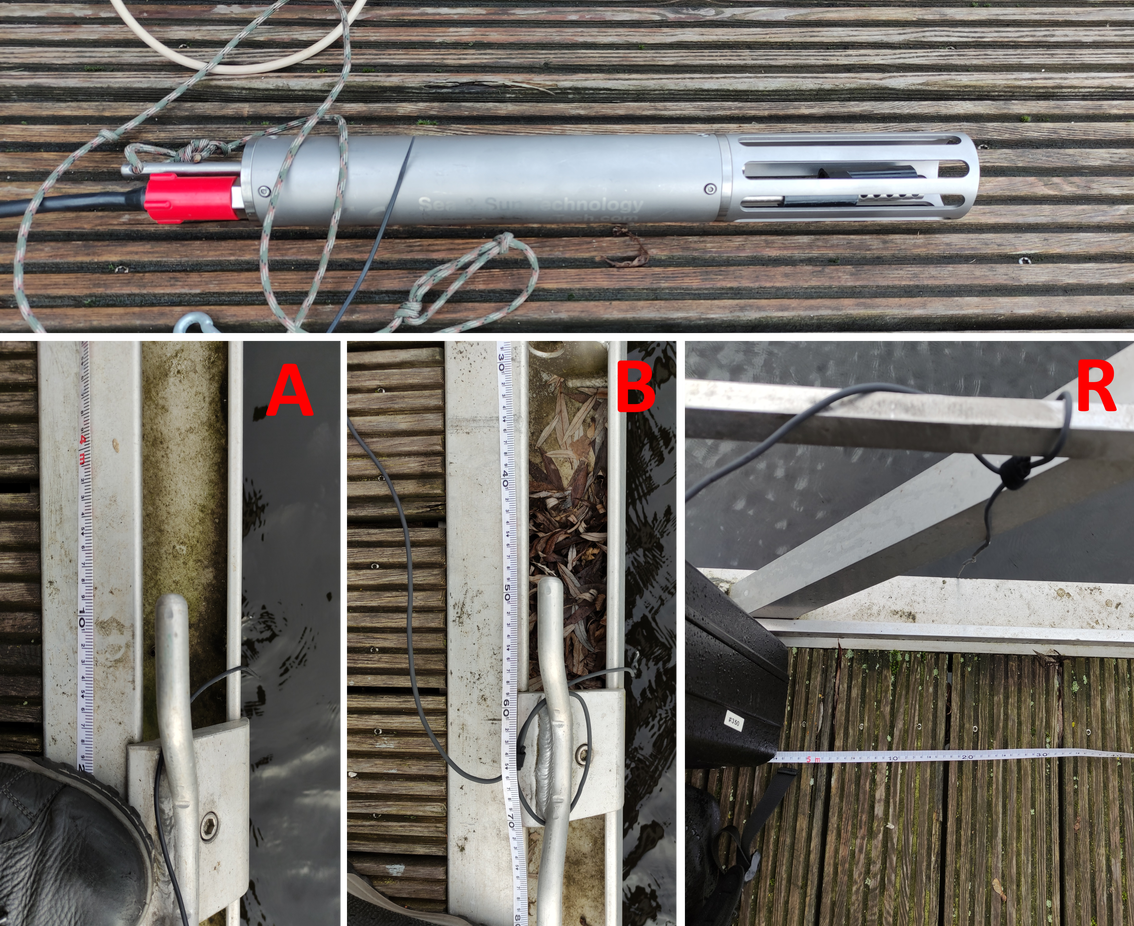
\includegraphics[width=12cm]{images/measurerealcomp}
	\caption{Location of field test, the markings represent the positions of the hydrophones. From left to right: receiver, sending anchor B and A. The CTD Sensor is depicted in the middle.}
	\label{fig:simsig}
\end{figure}
The figures presented here show the measured and expected values of a position over time for a standard and decreased signal strength for all three degrees of code.

\begin{figure}
	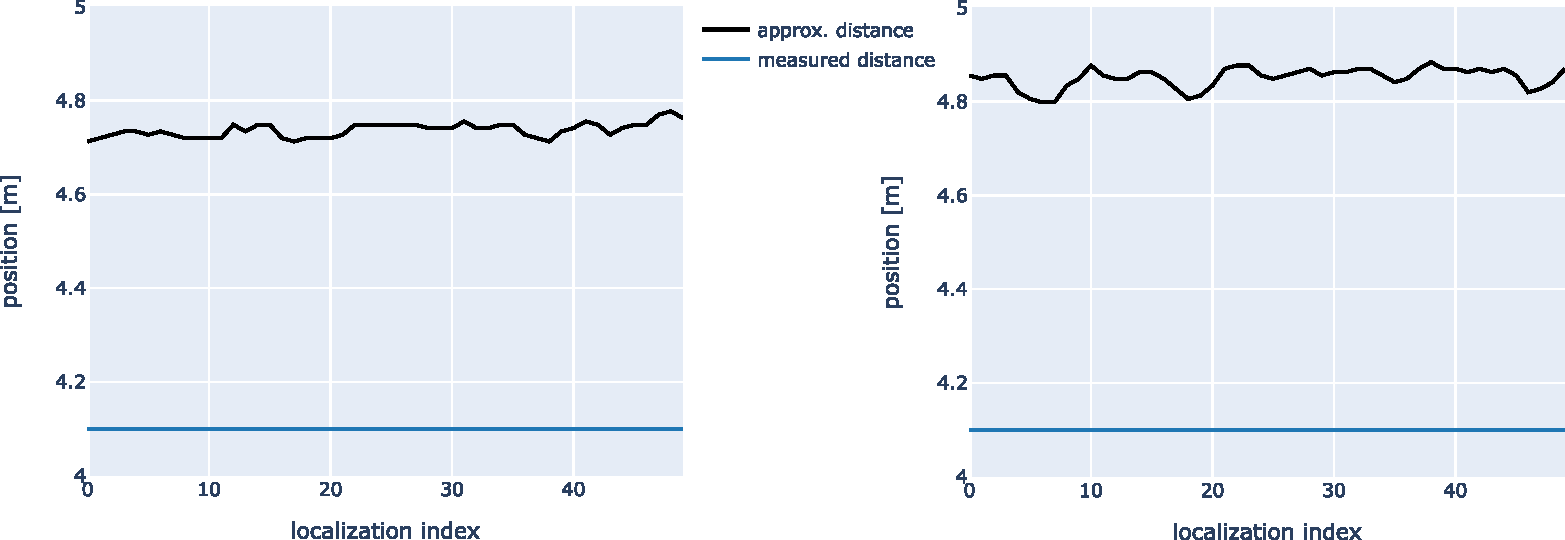
\includegraphics[width=\linewidth]{images/d10fvsd10fn} 
	\caption{Evaluation of 10th degree code. High SNR at the left and low SNR at the right.}
	\label{fig:d10fvsd10fn}
\end{figure}
It is observed that with a code of 10th degree, there is a significant offset of approximately \SI{60}{\centi\meter} between the measured and expected values \ref{fig:d10fvsd10fn}. This offset is likely a result of synchronization problems between the oscilloscopes used in the experiment. However, it is also worth noting that despite this offset, the position demonstrates a high degree of stability with minimal variations of less than \SI{10}{\centi\meter}. Additionally, by decreasing the SNR, it is observed that the position is shifted somewhat by under \SI{20}{\centi\meter}. In conclusion, this demonstrates that despite the offset, the overall position remains relatively consistent.
\begin{figure}
	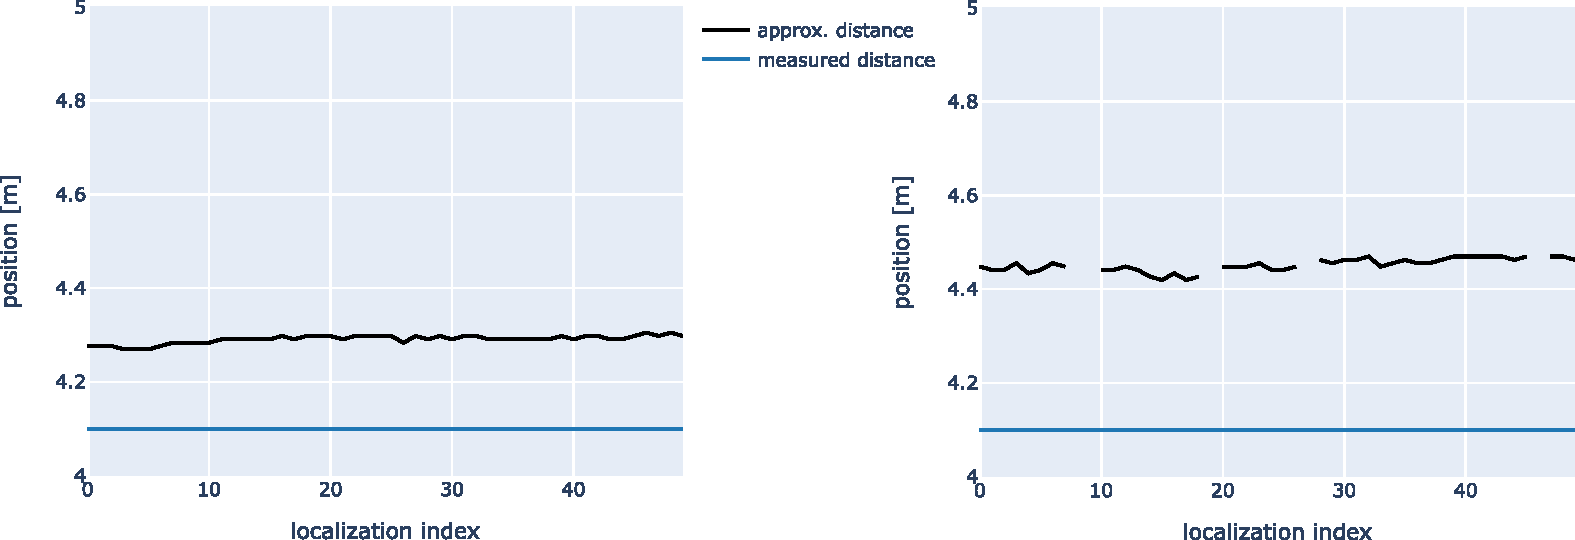
\includegraphics[width=\linewidth]{images/d9fvsd9fn} 
	\caption{Evaluation of 9th degree code}
	\label{fig:d9fvsd9fn}
\end{figure}
The next measure presents the results of the position measurement when the code of 9th degree is used. It is observed that when the default SNR is in use, similar results are obtained as with codes of 10th degree. However, when the SNR is decreased, the peak detection fails \ref{fig:d9fvsd9fn}. This is an important issue to consider, as the ability to accurately detect peaks is crucial for obtaining accurate position measurements. Additionally, values outside the interval from $4$ to $5$ were excluded. The failure of peak detection in this measure is likely due to the enlarged sidelobes, which are known to distract the CFAR algorithm. As a result, the performance of the system is worse compared to when the code is at 10 degrees. This highlights the importance of maintaining a high SNR and the potential impact of sidelobes on the performance of the algorithm.

\begin{figure}
	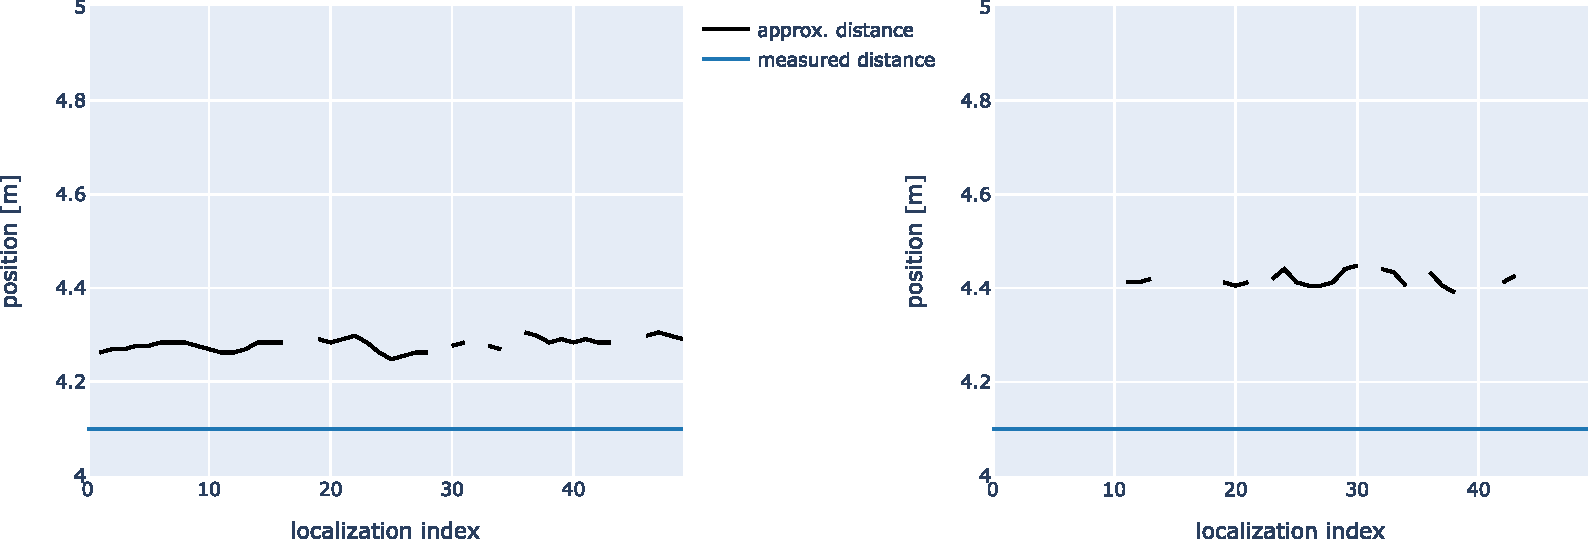
\includegraphics[width=\linewidth]{images/d8fvsd8fn}
	\caption{Evaluation of 8th degree code}
	\label{fig:d8fvsd8fn}
\end{figure}

The final measure presents the results of the position measurement with code of 8th degree. It is observed that this measure follows the downwards trend of performance that was previously noted with code of 9th degree. Specifically, it is found that both low and high SNR position detection's could not be completed without outliers resulting from failed peak detection \ref{fig:d8fvsd8fn}. This further emphasizes the importance of maintaining a high SNR and the potential impact of sidelobes on the performance of the algorithm.

\begin{tuhhtable}
	\centering
	\begin{tabular}[tp]{C{.2\linewidth}C{.2\linewidth}R{.2\linewidth}R{.2\linewidth}}
		\THc{1}{c}{code degree} & \THc{1}{c}{SNR} & \THc{1}{c}{fasle alarm rate} & \THc{1}{c}{minimum theshold} \\
		\abovebodyrule
		10 &  high & 9\% & 0.2 \\\TRc
		10 &  low & 12\% & 0.4 \\
		\hline
		9 &  high & 12\% & 0.2 \\\TRc
		9 &  low & 17\% & 0.4 \\
		\hline
		8 &  high & 26\% & 0.4 \\\TRc
		8 &  low & 26\% & 0.4 \\
		\belowbodyrule
	\end{tabular}
	\caption{Used false alarm rate and minimum threshold in CFAR for different degrees and SNR's}
	\label{tbl:degfarsnr}
\end{tuhhtable}
It is important to note that the false alarm rate and the minimum threshold of the CFAR algorithm must be adjusted to maintain successful peak detection in varying code degrees and SNR levels. As code degree and SNR decrease, the false alarm rate and minimum threshold must be increased to compensate for decreased system performance \ref{tbl:degfarsnr}.

In conclusion, the results of these measures demonstrate the importance of maintaining a high SNR for accurate peak detection and position measurement. As the code degree decreases, the performance of the system worsens, highlighting the need for codes of higher degrees to achieve better results. Additionally, a small shift in position under \SI{20}{\centi\meter} is observable on all results when the SNR is decreased, emphasizing the importance of a high SNR in maintaining the accuracy of the position measurements.

\chapter{Localization}

\section{Peak detection}

The received signal, consisting of summed delayed signals, cross-correlated by every anchor. If the signal is not reflected the peak in cross-correlation would be obvious. But because by the introduction of noise and water reflections a higher rate of similar peaks appear. To suppress these effects a CA-FAR Algorithm \cite{rohling11} is applied to only detect the first reflected peak resulting in lower false alarms of peaks. \\
CA-FAR works by using multiple values intervals. The most outer one could be described as a train bin and is used to get an estimation of the signals noise. Especially CA-FAR uses averaging to estimate the noise by measured cells. The bordering bin, defined as the guard cells, is used to reduce self-interference of the peaks. Thus, increasing window sizes $W$ results in better noise estimating but overall detectability is still limited by the sample rate  \cite{rohling11}\cite{radarbasics}. By knowledge of measured peak widths a optimal guard interval can be figured.\\
The calculated threshold is than scaled by a formula depending on the false alarm rate. The higher the false alarm rate, the weaker high amplitude peaks gets included by the estimated threshold \ref{eq:cff}.\\
%Because Cell Averaging shows not satisfactory results in sensitive multi targets examples, the noise estimation could be enhanced by a sorting average applied to the %train interval. That principle is defined as CO-FAR \cite{rohling11}. 
%\begin{center}
%	\begin{tabular}{|c|c|}
%			\hline
%			candidate sample & $i$\\
%			\hline
%			guard interval (half) & $\mathcal{G}$ \\
%			\hline
%			train interval (half) & $\mathcal{T}$ \\
%			\hline
%			false alarm rate & $\eta$\\
%			\hline
%		\end{tabular}
%	\linebreak
%\end{center}
%
%\begin{equation}
%	Threshold(i)_x=
%	\cfrac{\alpha}{2\mathcal{T}}
%	\left[ \sum_{j=i-\left( \mathcal{G}+\mathcal{T}\right) }^{i+\left( \mathcal{G}+\mathcal{T}\right)}x(j) - \sum_{j=i-\mathcal{G}}^{i+\mathcal{G}}x(j) \rigbest NAht] 
%	\label{eq:cft}
%\end{equation}
%\begin{equation}
%	\text{scale factor}~~~
%	\alpha=2\mathcal{T}\left( \eta^{-1/{2\mathcal{T}}}-1\right) 
%	\label{eq:cff}
%\end{equation}
\begin{figure}[h]
	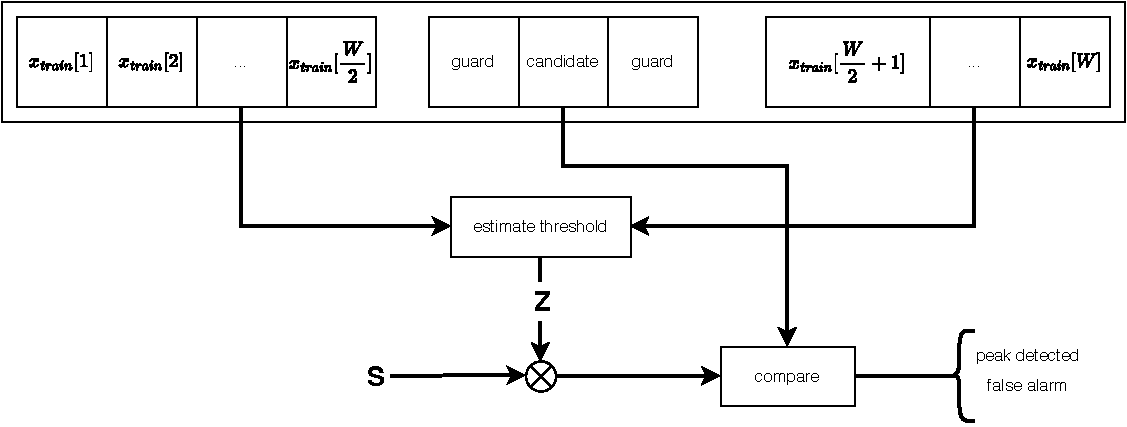
\includegraphics[width=\linewidth]{images/peakdet}
	
	\caption{CFAR threshold peak detection procedure \cite{rohling11}}
	\label{fig:simsig}
\end{figure}

\begin{equation}
	T=S\cdot Z,~~~Z_{CA}=\sum_{i=1}^{W}\dfrac{1}{W}x_{train}
	\label{eq:cff}
\end{equation}


\section{Explicit Position calculation}

The initial condition for the localization are four anchors $S_i$ with thir coordinates $\{x_i,y_i,z_i\}$ and the target $S$ which is to be located. By multiplying relative delays by the speed of sound $c$ which is approximately set to $1500\,\frac{m}{s}$, the distance $d_{ij}$ between the reference anchor $S_0$ and $S_i$ is calculated.\\
\begin{equation}
	d_{ij}=c\cdot\tau_{ij}=c\cdot (t_i-t_j),~~~\text{absolute delays } t_k,~k\in \{0,1,2,3\}
\end{equation}
By these values a Matrix $A$ and vector $\vec{b}$ is created. Thus, a System $A\cdot \vec{x}=\vec{b}$ is established. This linear system can be solved by using the inverse method if Matrix $A$ has full rank. Otherwise least squared can be used but yields undesirable results. In three dimensional Space five anchors are needed for full rank. The solution $\vec{x}$ are the coordinates $\{x,y,z\}$ of the target $S$ \cite{yang11}.

\begin{equation}
	A=\left[
	\begin{array}{cccc}
		x_0-x_1 & y_0-y_1 & z_0-z_1 & d_{01}\\
		x_0-x_2 & y_0-y_2 & z_0-z_2 & d_{02}\\
		x_0-x_3 & y_0-y_3 & z_0-z_3 & d_{03}\\
		x_0-x_4 & y_0-y_4 & z_0-z_4 & d_{04}\\
	\end{array}
	\right]
\end{equation}
\begin{equation}
	\vec{b}=\cfrac{1}{2}\left[
	\begin{array}{c}
		x_0^2-x_1^2+y_0^2-y_1^2+z_0^2-z_1^2+d_{01}^2\\
		x_0^2-x_2^2+y_0^2-y_2^2+z_0^2-z_2^2+d_{02}^2\\
		x_0^2-x_3^2+y_0^2-y_3^2+z_0^2-z_3^2+d_{03}^2\\
		x_0^2-x_4^2+y_0^2-y_4^2+z_0^2-z_4^2+d_{04}^2\\
	\end{array}
	\right]
	,~~~
	\vec{x}=\left[
	\begin{array}{c}
		x\\
		y\\
		z\\
		||S-S_0||_2\\
	\end{array}
	\right]
\end{equation}
Theoretically an system $A$ of lower rank can be solve by least squares. Having said this, positions calculated by that approach could not satisfy the demands of 3D localization.

\begin{equation}
	\vec{x}=(A^T A)^{-1} A^T\vec{b}
\end{equation}

\section{GPS like localization method}

Because of restrictions introduced in the the first localization method an alternative localization procedure is probed. Thus a position calculation by four anchors is alternatively pursued.\\
\begin{equation}
	x_{ji}:=x_j-x_i,~~~~~
	y_{ji}:=y_j-y_i,~~~~~
	z_{ji}:=z_j-z_i~~~~~
\end{equation}
By rearranging the derivation of hyperbola intersections the following substitutes can be defined. 
\begin{equation}
	\mathbf{A}=\cfrac{d_{02}x_{10}-d_{01}x_{20}}{d_{01}y_{20}-d_{02}y_{10}},~~~
	\mathbf{B}=\cfrac{d_{02}z_{10}-d_{01}z_{20}}{d_{01}y_{20}-d_{02}y_{10}}
\end{equation}	
\begin{equation}
	\mathbf{C}=\cfrac{d_{02}\left(d_{01}^2+x_0^2-x_1^2+y_0^2-y_1^2+z_0^2-z_1^2\right)-d_{01}\left(d_{02}^2+x_0^2-x_2^2+y_0^2-y_2^2+z_0^2-z_2^2\right)}{2\left(d_{01}y_{20}-d_{02}y_{10}\right)}
\end{equation}	

\begin{equation}
	\mathbf{D}=\cfrac{d_{23}x_{12}-d_{21}x_{32}}{d_{21}y_{32}-d_{23}y_{12}},~~~
	\mathbf{E}=\cfrac{d_{23}z_{12}-d_{21}z_{32}}{d_{21}y_{32}-d_{23}y_{12}}
\end{equation}	
\begin{equation}
	\mathbf{F}=\cfrac{d_{23}\left(d_{21}^2+x_1^2-x_1^2+y_1^2-y_1^2+z_0^2-z_1^2\right)-d_{21}\left(d_{23}^2+x_1^2-x_2^2+y_1^2-y_2^2+z_1^2-z_2^2\right)}{2\left(d_{21}y_{32}-d_{23}y_{12}\right)}
\end{equation}	

\begin{equation}
	\mathbf{G}=\cfrac{\mathbf{E}-\mathbf{B}}{\mathbf{A}-\mathbf{D}},~~~
	\mathbf{H}=\cfrac{\mathbf{F}-\mathbf{C}}{\mathbf{A}-\mathbf{D}},~~~
	\mathbf{I}=\mathbf{A}\cdot \mathbf{G}+\mathbf{B},~~~
	\mathbf{J}=\mathbf{A}\cdot \mathbf{H}+\mathbf{C}
\end{equation}	

\begin{equation}
	\mathbf{K}=d_{02}^2+x_0^2-x_2^2+y_0^2-y_2^2+z_0^2-z_2^2+2x_{20}\mathbf{H}+2y_{20}\mathbf{J}
\end{equation}	

\begin{equation}
	\mathbf{L}=2\left(x_{20}\mathbf{G}+y_{20}\mathbf{I}+z_{20}\right)
\end{equation}	

\begin{equation}
	\mathbf{M}=4d_{02}^2\left(\mathbf{G}^2+\mathbf{I}^2+1\right)-\mathbf{L}^2
\end{equation}	

\begin{equation}
	\mathbf{N}=8d_{02}^2\left[\mathbf{G}\left(x_0-\mathbf{H}\right)+\mathbf{I}\left(y_0-\mathbf{J}\right)+z_0\right]+2\mathbf{L}\cdot\mathbf{K}
\end{equation}	

\begin{equation}
	\mathbf{O}=4d_{02}^2\left[\left(x_0-\mathbf{H}\right)^2+\left(y_0-\mathbf{J}\right)^2+z_0^2\right]-\mathbf{K}^2
\end{equation}	

A downside of this approach is the uncertainty of position $z$. Thus, additional information on bounds is necessary. The target won't get above sea level. Consequently, at least one boundary $z_{surface}$ which acts like a maximum can be set. The minimum value $z_{ground}$ can be assumed as the lowest position achievable underwater. 
\begin{equation}
	z_{a,b}=\cfrac{\mathbf{N}}{2\mathbf{M}}\pm\sqrt{\left(\cfrac{\mathbf{N}}{2\mathbf{M}}\right)^2-\cfrac{\mathbf{O}}{\mathbf{M}}}
\end{equation}	

\begin{equation}
	z=\min\left\{\max\left\{z_a,~z_b,~z_{surface}\right\},~z_{ground}\right\}
\end{equation}	

The resulting x and y values of our target can then be calculated by the following formula using the selected $z$.

\begin{equation}
			\vec{x}
	=\left[
	\begin{array}{c}
		x\\
		y\\
		z
	\end{array}
	\right]
=\left[
	\begin{array}{c}
		\mathbf{G}z+\mathbf{J}\\
		\mathbf{I}z+\mathbf{H}\\
		z
	\end{array}
	\right]
\end{equation}	

\chapter{Conclusion}
In this research project, the optimal orthogonal pseudorandom code, named gold codes, have been selected due to their satisfactory correlation properties and scalability. The signal processing, which includes modulation, filtering, and peak detection, has been successfully implemented in python. As a result, a 3D position localization algorithm has been developed that operates effectively in a simulated environment with only 4 anchors.

To sum up the evaluation, the results of the data in this research project have demonstrated the effectiveness of using orthogonal codes for acoustic underwater localization. The simulation results have shown a stable localization performance, with higher SNR levels resulting in improved stability in peak detection. The principle of sidelobe increase has been observed to have a significant impact on the localization performance at lower SNR levels. The field testing results have confirmed the stability of the localization performance, particularly for codes of 10th degree. The CA-FAR algorithm has been found to be an effective tool for peak detection, but its performance still needed improvements by adjusting its false alarm rate based on the SNR and code degree.

In terms of future research, there is room for improvement in the CFAR algorithm, such as the use of sorted data bins (OS-CFAR). Besides that, also alternative peak detection method could be tested in combination with CFAR.

Moreover, exploring other options for increasing the gold code length, such as a method for concatenating codes without negatively impacting their correlation properties, could be investigated in future studies. This would provide more opportunities for improving the localization performance and may achieving even higher noise and multipath propagation tolerances. 

Additionally, the effectiveness of the simulated setup with four anchors for 3D position localization, such as with the BlueROV2 underwater vehicle, could be further evaluated in real-world scenarios to gain a better understanding of its practical performance and limitations.
% The Chapters
%\chapter{Introduction}

This documents describes the usage and features of the TUHH Telematics Thesis Class for \LaTeX. While the intention of this work is to explain the class and its functions to you, it is far from being complete or exhaustive. You are most welcome to contribute to this class and the attached packages by sending enhancements or feature proposals to \texttt{christian.renner@tu-harburg.de}. In case of any questions, feel also free to send an E-Mail.




%\chapter{Structure}

This chapter is intended to give you an overview about structuring your work. Note that the following instructions must be understood as a guideline. Of course, the final structure of your thesis report depends on the actual nature of the topic. For instance, the structure of pure theoretical work differs from that of implementational ones. Before starting structuring your work, discuss the actual content, chapters and sections with your supervisor.

\section{...}

Ok, this piece of writing is incomplete ... and reserved for some future version of this guide ...
%\chapter{The TUHH Telematics Thesis Class}

In order to free you from reading through all the classes and packages provided with our Thesis Template, we will summarize the main parts for you. The root document of your thesis is the file \file{thesis.tex}. It contains global setup and the inclusion of the different chapters, which are outsourced to individual files, i.e., each chapter is organized in a dedicated file.

\section{Setup}

Before starting your thesis report, adjust all the personal and thesis related data in the root document. We will briefly cover this matter.


\subsection{Options}\label{sub:options}

If you have at look at the very first line of the root document, you'll discover the loaded document class along with its options. The most important options are:
\begin{description}
  \item[de] German Version (cannot be combined with option \texttt{en})
  \item[en] English Version, default (cannot be combined with option \texttt{de})
  \item[gray] Use this option to make a gray-style version of the thesis report
  \item[print] Use this option for your print version, i.e, switched off hyperref colors (this makes only sense for electronic versions)
  \item[declaration] Use this option for inclusion of the declaration by candidate
  \item[abstract] This option enables the automatic inclusion of an abstract, which is expected in the file \file{prelude\_abstract.tex}
  \item[acknowledgment] This option enables the automatic inclusion of an acknowledgment, which is expected in the file \file{prelude\_acknowledgment.tex}
  \item[symbollist] If you have a bunch of mathematical symbols, use this option in order to automatically include a list of symbols. The latter has to be provided the file \file{prelude\_symbols.tex}
  \item[cv] Use this option to include your curriculum vitae at the end of the document. The latter has to be provided the file \file{postlude\_cv.tex}. This is required for PhD theses.
  \item[ownpub] Use this option to include a list of your own publications. The latter has to be provided the file \file{ownpub.bib}. This is required for PhD theses. Make sure to also run \texttt{bibtex ownpub}, otherwise your own publications will not show up.
\end{description}


\subsection{Thesis Type}

Depending on the actual type of thesis, you have to use the correct parameter for the command \cmd{\textbackslash{}setthesistype}: \emph{bachelorthesis}, \emph{projectwork}, \emph{masterthesis}, \emph{diplomathesis}, and \emph{phdthesis}.


\subsection{Author, Title, and Date}

Next, you must specify your name, your matriculation number and course of studies, along with the title of the thesis, and the date of submission with the corresponding commands \cmd{\textbackslash{}author}, \cmd{\textbackslash{}matrnumber} \cmd{\textbackslash{}course}, \cmd{\textbackslash{}title}, and \cmd{\textbackslash{}date}. The latter of these takes two arguments: the actual, complete date of submission and a short version for the title page with month and year only.

A PhD thesis also requires the following values: 
\cmd{\textbackslash{}submitdate}, \cmd{\textbackslash{}setBirthplace} and \cmd{\textbackslash{}setPhDType}. The latter must be one of the values \emph{ing}, \emph{nat}, or \emph{pol}.

\subsection{Institute, Supervisor, and Examiner}

You can set up one or two examiners for your thesis, depending on the examination regulations for your thesis. This is done via the commands
\cmd{\textbackslash{}examinerFirst} and \cmd{\textbackslash{}examinerSecond}. Each of these takes two parameters: the name of the examiner and his or her affiliation, i.e., the institute and university (the latter two should be separated by \cmd{\textbackslash{}newline}).
You may also provide up to two supervisors (tutors) of your thesis. This is done via the commands \cmd{\textbackslash{}supervisorFirst} and \cmd{\textbackslash{}supervisorSecond}. The command requires the same two parameters as the examiner commands. However, the affiliation should make up a single line, i.e., separate institute and university by commas.
Finally, you have to specify the institute explicitly using the command \cmd{\textbackslash{}institute}. Available parameters are defined in the file \file{tuhhlangnames.def}. Most likely, you will need \emph{InstTelematics}.


\section{Building Blocks}

Your report consists of a couple of building blocks, which we will discover and explain in this section.


\subsection{Mathematical Symbols}

At the moment, there is one major hint for you: If there are going to be any mathematical symbols in your report, define a command for each of them in the file \file{setup\_math.tex}. First of all, this makes your sourcecode---and equations in particular---more readable. Secondly, symbols can be replaced or altered quickly and elegantly.

After the table of contents and before the first chapter of your report, show a table of all (mathematical) symbols used in your report with a brief explanation. An example is found in this document. Inclusion of such a list is explained in Sect.~\ref{sub:options}.


\subsection{Chapters}

Each chapter of your thesis should reside in a dedicated file. These files are linked into the thesis report via the \cmd{\textbackslash{}input} command. We do not discuss this matter in detail, but refer to the source code of this guide.


\subsection{Bibliography}

Since you're using \LaTeX, it's most suitable to employ BibTeX for your bibliography. By default, the bibliography is expected in the file \file{thesis.bib}. The specified style is a sincere recommendation. Information on required fields for the most important types of bibliography entries is provided in Sect.~\ref{sec:bib}.


\subsection{Appendix}

The appendix is organized as are the chapters: in separate files. In general, there should rarely be any need for a vast appendix. We only require you to have one appendix chapter for an attached CD/DVD with all your material, source code and the final versions (PDF) of your report and talk. If there are a few things that are related to your work, but do not suit into the main part, then these may go to the appendix. However, ask your supervisor before creating an appendix.


\subsection{Graphics and Plots}

If possible, try to draw your graphics with TikZ and the plots with Gnuplot with the TikZ terminal. TikZ is flexible, neat, and capable of using just the same fonts and symbols as used in and throughout your report. In general, create individual PDFs for each plot or graphic and insert it into your report using \cmd{\textbackslash{}includegraphics}. Doing so will speed up the compilation process. Ask your supervisor in case of any questions.


%\chapter{Figures, Tables, and more}

In this chapter, figures, tables, and listings as available in this template are being introduced.


\section{Figures}\label{sec:figures}

Figures should be frequently used throughout your thesis report, as they are a powerful instrument. Not only that one picture every two to three pages lightens up the work, a picture can even say more than a thousand words. However, note that a lonely figure is truly worthless. Make sure that you reference your figures in the text and that you explain them appropriately.

In the following, a set of useful commands for including figures into your work is introduced. Note that figures will be automatically placed by \LaTeX. You can rearrange figures be simply changing their position in the source code; however, you should not mess around with the figure placement options.


\subsection{Default yet Fancy Figures}\label{sub:simpleFigures}

Figures may require different display properties, so that a variety of different display styles are available. The main type of figures are illustrations. For these, the \cmd{\textbackslash{}fig} command is available. It has three parameters, which are the path to the picture, the caption, and the label. Labels of figures should have the prefix \cmd{fig:}. An example is shown in Figure~\ref{fig:simpleFigure}. The figure must be transparent, as it will be placed within a gray frame with a tiny border.

\fig{images/app_setup}{Figure with gray background box and border spacing. In this example, you also see what happens in case of a long caption.}{fig:simpleFigure}

In general, figures are displayed with a small inner spacing to the surrounding frame. As this may not be desired in some cases, there exists a version without additional spacing, \cmd{\textbackslash{}fignospacing}.


\subsection{The Frameless Variant}\label{sub:framelessFigures}

If you want to display photographs or illustrations, the surrounding frame and the gray background may be disturbing. Here, the command \cmd{\textbackslash{}fignoframe} jumps in and helps you out. The parameters are the same as described in Sect.~\ref{sub:simpleFigures}. See Fig.~\ref{fig:fignoframe} for a sample display.

\fignoframe{images/harvester}{Figure without surrounding frame and without gray background}{fig:fignoframe}


\subsection{Subfigures}\label{sub:subfigures}

When you start writing your evaluation and intend to display plots, having one plot per figure box is not a very handsome solution. Usually, you want to display multiple plots per figure box. This can be easily achieved using subfigures. In order to employ the neat and fancy boxing around your figures, use the \cmd{\textbackslash{}subfigbox}. As its first parameter, it takes a series of subfigures---using the \cmd{\textbackslash{}subfigure} command. Multiple rows are created using the \cmd{\textbackslash\!\textbackslash{}} command, automatic horizontal alignment is achieved via a \cmd{\textbackslash{}hfill} between adjacent figures in the same row. A possible layout is shown in Fig.~\ref{fig:trees}.

\subfigbox{
  \subfigure[complete]{\label{subfig:treeComplete}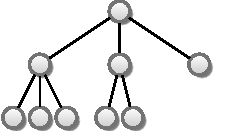
\includegraphics{images/tree_complete.pdf}}\hfill%
  \subfigure[min depth]{\label{subfig:treeMinDepth}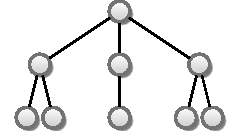
\includegraphics{images/tree_mindepth.pdf}}\hfill%
  \subfigure[full tree]{\label{subfig:treeFull}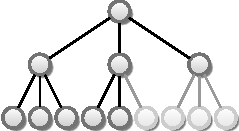
\includegraphics{images/tree_full.pdf}}%
}{Box with gray background intended to hold subfigures}{fig:trees}


%%
\section{Tables}\label{sec:tables}

Unfortunately, tables can be a pain in \LaTeX{} and have a clear tendency to look ugly. For this reason, we built the package \emph{tuhhtable}. A brief discussion of frequently used table pattern follow in dedicated subsections. 


\subsection{Simple Tables with Headings}\label{sub:simpleTables}

When creating tables, a couple of rules should be obeyed. Firstly, vertical lines are rarely helpful in tables. In contrast, they make a table harder to read in most cases, when people read from left to right. So try not to use them. To further support readability---while also hinting at eye candy---shaded rows are employed. To mark the end of a table and to separate the table body from the header, horizontal lines can be used. A recommended table layout is depicted in Table~\ref{tbl:simple}. Have a look at the source code of this document to understand how things work.

\begin{tuhhtable}
  \begin{tabular}[tp]{L{.3\textwidth}C{.3\textwidth}R{.3\textwidth}}
    \THc{1}{c}{Head 1} & \THc{1}{c}{Head 2} & \THc{1}{c}{Head 3} \\
    \THsub{1}{c}{sub 1} & \THsub{1}{c}{sub 2} & \THsub{1}{c}{sub 3} \\
    \abovebodyrule
    l1     & c1     & r1     \\\TRc
    l2     & c2     & r2     \\
    l3     & c3     & r3     \\\TRc
    \belowbodyrule
  \end{tabular}
  \caption{A simple table with a heading}
  \label{tbl:simple}
\end{tuhhtable}


\subsection{Special Table Elements}\label{sub:specialTableElements}

In case your are carrying out comparisons of, lets say, different algorithms, you might want to judge the quality of certain properties by symbols, such as '+', '-', or the like. Unfortunately, these symbols are not very fancy, so that we have defined a set of more eye-catchings ones. They are displayed in Table~\ref{tbl:elements}. Again, have a look at the source code of this document to understand how they can be used.

\begin{tuhhtable}
  \footnotesize\centering
  \begin{tabular}[tp]{L{.22\textwidth}C{.22\textwidth}C{.22\textwidth}C{.22\textwidth}}
    \THempty & \THc{1}{c}{Product 1} & \THc{1}{c}{Product 2} & \THc{1}{c}{Product 3} \\
    \abovebodyrule
    \TRh{1}{l}{has feature}  & \tblYes    & \tblYes  & \tblNo    \\\TRc
    \TRhc{1}{l}{usability}   & \tblGood   & \tblBest & \tblBad   \\
    \TRh{1}{l}{price}        & \tblNA     & \tblFair & \tblWorst \\\TRc
    \belowbodyrule
  \end{tabular}
  \caption{Special symbols for use in tables}
  \label{tbl:elements}
\end{tuhhtable}



\subsection{Advanced Tables}\label{sub:advancedTables}

Sometimes, a simple table layout as presented in the previous section is not sufficient. An example is shown in Table~\ref{tbl:advanced}. Hence, additional commands are available. 

% DECISION GUIDANCE TABLE
\begin{sidewaystable}
  \footnotesize\centering
  \begin{tabular}[htp]{lC{3.2cm}C{3.2cm}C{3.2cm}C{3.3cm}C{3.2cm}}
  \THempty    & \THc{1}{c}{Type I}   &
                 \THc{1}{c}{Type II}  &
                  \THc{1}{c}{Type III} &
                   \THc{1}{c}{Type IV}  &
                    \THc{1}{c}{Type V}  \\
%
  \TRx{6}{l}{Network Size}\\
  \abovebodyrule
  Small       & \tblWorst    & \tblGood     & \tblBest     & \tblBest     & \tblBad      \\\TRc
  Medium      & \tblFair     & \tblFair     & \tblGood     & \tblFair     & \tblFair     \\
  Large       & \tblBad      & \tblWorst    & \tblWorst    & \tblWorst    & \tblBest     \\
  \belowbodyrule
%
  \TRx{6}{l}{Density}\\
  \abovebodyrule
  Low         & \tblWorst    & \tblFair     & \tblBad      & \tblWorst    & \tblBad      \\\TRc
  Medium      & \tblFair     & \tblFair     & \tblFair     & \tblFair     & \tblGood     \\
  High        & \tblWorst    & \tblFair     & \tblGood     & \tblFair     & \tblGood     \\
  \belowbodyrule
%
  \TRx{6}{l}{Initial Fill Level}\\
  \abovebodyrule
  Low         & \tblFair     & \tblGood     & \tblBest     & \tblBest     & \tblGood     \\\TRc
  High        & \tblBad      & \tblBad      & \tblWorst    & \tblWorst    & \tblBest     \\
  \belowbodyrule
%
  \TRx{6}{l}{Variation of Initial Fill Levels}\\
  \abovebodyrule
  Low         & \tblBest     & \tblGood     & \tblBad      & \tblGood     & \tblBest     \\\TRc
  High        & \tblBest     & \tblBad      & \tblWorst    & \tblGood     & \tblBest     \\
  \belowbodyrule
%
  \TRx{6}{l}{Collisions and Packet Loss}\\
  \abovebodyrule
  Collisions / Yield &
    \tblYes / \tblWorst &
    \tblNo  / \tblBest &
    \tblNo  / \tblBest &
    \tblNo  / \tblBest &
    \tblYes / \tblFair     \\\TRc
  Packet Loss & \tblGood     & \tblFair     & \tblWorst    & \tblWorst    & \tblGood     \\
  \belowbodyrule
  \end{tabular}
  \caption{Characteristics of the TDMA schedules: Decision Guidance \cite{Renner:2008:Diploma}}
  \label{tbl:advanced}
\end{sidewaystable}



\section{Enumerations \& Co.}\label{sec:enumerations}

Feel free to use enumerations, itemizations, and the like to suit your needs. We have adjusted the itemization to match our slides class plus our color scheme. We thus discourage you from changing items or colors.



\section{Listings}\label{sec:listings}

For placing and typesetting listings, we encourage the use of the \emph{listings} package available for \LaTeX. Please have a look into the corresponding package manual. The facilitate the usage of this package, we have already set it up to follow the same look as the rest of our visual stuff. This includes the gray background, the frame, and appropriate colors. The package is automatically loaded by the template class and defines \emph{C++} as the default programming language---you are completely free to adjust the language, of course. A sample listing is displayed in Lst.~\ref{lst:sampleListing}. Note that all listings should have labels with the prefix \cmd{lst:} and should be referenced in the text. Besides complete listings, we have defined the command \cmd{\textbackslash{}cmd}, which display its first parameter text in monospace font.

\begin{tuhhlisting}[label=lst:sampleListing,caption={A simple C++ program for reading in positions},language=C++]
#include <iostream>                                                                       
#include <vector>                                                                         
#include <inttypes.h>                                                                     

using namespace std;

/* 2-D positions */
typedef struct pos_s {
        int16_t  x, y;
} pos_t;

int main(void)
{
        uint16_t       numData;
        vector<pos_t>  v;
        pos_t          tmp;

        /* read numData 2-D points */
        cin >> numData;
        for (unsigned i = 0; i < numData; i++) {
                cin >> tmp.x >> tmp.y;
                v.push_back(tmp);
        }
        cout << "read " << numData << " points" << endl;

        /* process data */
        process(v);

        return 0;
}
\end{tuhhlisting}

%\chapter{Style Guide}\label{cha:styleGuide}

Finally, we want to give some advices and recommendations on styling. This does not relate to writing skills, which is gracefully embraced by the \emph{Chicago Writer's Manual}.


\section{Fonts}\label{sec:fonts}

Font setup etc. has been done for you by means of this very template. We hence expect you to follow the given style; meaning that we discourage you from changing font sizes, faces, families, colors, as well as line and paragraph spacing or any spacing in general.


\section{Citing and Referencing}\label{sec:citeAndRef}

Citing other sources and referencing parts of your work is quite easy using the commands \cmd{\textbackslash{}cite} and \cmd{\textbackslash{}ref}. Yet, let us mention some aspects. Firstly, when citing, you should make clear, somehow, which part is from the cited work and which is not. Secondly, you most likely want to place a tilde ($\sim$) between the word just in front of the \cmd{\textbackslash{}cite} or \cmd{\textbackslash{}ref} commands to avoid ugly looking line breaks. Thirdly, note that citations and references are proper parts of a sentence: Do not simply put them at the end of a sentence; use them as nouns!

More importantly, obey the following rules. Always capitalize when referencing, e.g., say Fig.~17 instead of fig.~17. You can abbreviate Figure with Fig., Section with Sect., and Listing with Lst. When referencing equations, simply place the number in parentheses---e.g., say (3.2) instead of Eq.~3.2---that's all. While you can certainly do this by hand, we encourage you to use the \emph{cleveref} package, which already does this for you. By using \cmd{\textbackslash{}cref} or \cmd{\textbackslash{}Cref} (at the beginning of a sentence) as a replacement for \cmd{\textbackslash{}ref}, the type of reference is automatically added. Please check the manual of the package for further details.

For your own sake, use a pattern for labels. We recommend to use prefixes for each type of label: chapters (\cmd{cha:}), sections (\cmd{sec:}), subsections and below (\cmd{sub:}), figures (\cmd{fig:}), tables (\cmd{tbl:}), listings (\cmd{lst:}), and equations (\cmd{eqn:}).


\section{Physical Units}\label{sec:siunits}

If you plan on using physical units, particularly SI-units, in your report, we encourage you to use the \emph{siunitx} package for \LaTeX. In all cases, separate numbers from their units with a small space, i.e., with a \cmd{\textbackslash{},}. Well, there is an exception: No space for~\%!


\section{Mathematical Stuff}

When using mathematical functions or sub-/superscripts that are text and not variables, please typeset these appropriately: In the case of functions, use the command version, e.g., \cmd{\textbackslash{}log} (prints $\log$) instead of plainly \cmd{log} (which prints $log$). For subscripts or the like, use the command \cmd{\textbackslash{}textnormal}. Compare $T_{sleep}$ with $T_\textnormal{sleep}$. The reasons for this is twofold. Firstly, the produced italic text looks ugly, and secondly, italics are used for variables (only).

The usage of the environment \cmd{equation} is disouraged and may cause display errors. In the future, please use the \cmd{align} environment for equations:

\begin{align*}
	|x|= 
	\begin{cases} 
			x 	& \text{if $x > 0 $,} \\
			-x 	& \text{if $x \leq 0$.}
	\end{cases}
\end{align*}

\begin{tuhhlisting}[language=TeX]
\begin{align*}
	|x|= 
	\begin{cases} 
			x 	& \text{if $x > 0 $,} \\
			-x 	& \text{if $x \leq 0$.}
	\end{cases}
\end{align*}
\end{tuhhlisting}



\section{Bibliography}\label{sec:bib}

When it comes to writing your bibfile, i.e., your bibliography, please follow the next few advices. Firstly, be consistent (if possible): Regarding authors' names, either abbreviate first names always or write them out always! For US addresses, write down the name of the city, the two-character abbreviation for the state plus the term USA! For all other countries, the name of the city and the country are sufficient. Capitalize titles correctly (there are multiple rules on this, please pick one and stick to it)! If possible, write down the full name of a conference and repeat its abbreviation with the year in parentheses afterwards. We give a few examples in the following listings.

Beside this, please have a look at the required fields for the main types of citations:
\begin{description}
  \item[Journal Articles] Use the type \cmd{@article} and include the fields \cmd{author}, \cmd{title}, \cmd{journal}, \cmd{volume}, \cmd{number}, \cmd{year}, \cmd{publisher}, and \cmd{address}.
  \item[Conference Papers] Use the type \cmd{@inproceedings} and provide the fields \cmd{author}, \cmd{title}, \cmd{booktitle}, \cmd{month}, \cmd{year}, and \cmd{address}.
  \item[Technical Reports] Use the type \cmd{@techreport} and provide the fields \cmd{author}, \cmd{title}, \cmd{month}, \cmd{year}, and \cmd{institution}.
  \item[Websites] Use the type \cmd{@misc} and provide the fields \cmd{author}, \cmd{title}, \cmd{year}, \cmd{note} and \cmd{howpublished}. The last two fields hold a note on your last visiting date of the site and its web address.
\end{description}

We have put together a couple of examples for you in Lst.~\ref{lst:sampleBibtex}.

\begin{tuhhlisting}[label=lst:sampleBibtex,language=TeX,caption={BibTeX examples},{morekeywords={@article,@inproceedings,@techreport,@misc}},{morestring=[b]"}]
@article{ ECPS:2002:ConnectingThePhysicalWorld,
	author       = "D. Estrin and D. Culler and K. Pister and G. Sukhatme",
	title        = "{Connecting the Physical World with Pervasive Networks}",
	journal      = "IEEE Pervasive Computing",
	volume       = "1",
	number       = "1",
	year         = "2002",
	publisher    = "IEEE Educational Activities Department",
	address      = "Piscataway, NJ, USA"
}

@inproceedings{ KPC:2006:StructuralMonitoring,
	author       = "S. Kim and S. Pakzad and D. Culler and J. Demmel and G. Fenves and S. Glaser and M. Turon",
	title        = "{Wireless Sensor Networks for Structural Health Monitoring}",
	booktitle    = "Proceedings of the 4th International Conference on Embedded Networked Sensor Systems (SenSys~'06)",
	month        = oct,
	year         = "2006",
	address      = "Boulder, CO, USA"
}

@techreport{ EV:2005:TDMAScheduling,
	author       = "S. Coleri Ergen and P. Varaiya",
	title        = "{TDMA Scheduling Algorithms for Sensor Networks}",
	year         = "2005",
	month        = jul,
	institution  = "Department of Electrical Engineering and Computer Science, University of California, Berkeley, CA, USA"
}

@misc{ TI5:WIKI,
	author       = "S. Untersch{\"u}tz",
	title        = "{Network Simulator (NS-2), Institute of Telematics, Hamburg University of Technology, Germany}",
	howpublished = "http://wiki.ti5.tu-harburg.de/wsn/ns2/intro",
	year         = 2008,
	note         = "Last visited: 05/06/2008"
}
\end{tuhhlisting}



% Bibliography
% if you have cited papers that are not referenced, but important for your work,
% uncommented the following line; however, this should generally by unnecessary
% and hints at improper citing.
%\nocite{*}
\tuhhbibliography{thesis}


% Appendix
% Feel free to add additional appendix chapters (e.g., measurement setups, etc.)
\begin{tuhhappendix}
  %\chapter{Content of the DVD}

In this chapter, you should explain the content of your DVD. 

  \chapter{Localization Formula}

\begin{equation}
	x_{ji}:=x_j-x_i,~~~~~
	y_{ji}:=y_j-y_i,~~~~~
	z_{ji}:=z_j-z_i~~~~~
\end{equation}

\begin{equation}
	{A}=\cfrac{d_{02}x_{10}-d_{01}x_{20}}{d_{01}y_{20}-d_{02}y_{10}},~~~
	{B}=\cfrac{d_{02}z_{10}-d_{01}z_{20}}{d_{01}y_{20}-d_{02}y_{10}}
\end{equation}	
\begin{equation}
	{C}=\cfrac{d_{02}\left(d_{01}^2+x_0^2-x_1^2+y_0^2-y_1^2+z_0^2-z_1^2\right)-d_{01}\left(d_{02}^2+x_0^2-x_2^2+y_0^2-y_2^2+z_0^2-z_2^2\right)}{2\left(d_{01}y_{20}-d_{02}y_{10}\right)}
\end{equation}	

\begin{equation}
	{D}=\cfrac{d_{23}x_{12}-d_{21}x_{32}}{d_{21}y_{32}-d_{23}y_{12}},~~~
	{E}=\cfrac{d_{23}z_{12}-d_{21}z_{32}}{d_{21}y_{32}-d_{23}y_{12}}
\end{equation}	
\begin{equation}
	{F}=\cfrac{d_{23}\left(d_{21}^2+x_1^2-x_1^2+y_1^2-y_1^2+z_0^2-z_1^2\right)-d_{21}\left(d_{23}^2+x_1^2-x_2^2+y_1^2-y_2^2+z_1^2-z_2^2\right)}{2\left(d_{21}y_{32}-d_{23}y_{12}\right)}
\end{equation}	

\begin{equation}
	{G}=\cfrac{{E}-{B}}{{A}-{D}},~~~
	{H}=\cfrac{{F}-{C}}{{A}-{D}},~~~
	{I}={A}\cdot {G}+{B},~~~
	{J}={A}\cdot {H}+{C}
\end{equation}	

\begin{equation}
	{K}=d_{02}^2+x_0^2-x_2^2+y_0^2-y_2^2+z_0^2-z_2^2+2x_{20}{H}+2y_{20}{J}
\end{equation}	

\begin{equation}
	{L}=2\left(x_{20}{G}+y_{20}{I}+z_{20}\right)
\end{equation}	

\begin{equation}
	{M}=4d_{02}^2\left({G}^2+{I}^2+1\right)-{L}^2
\end{equation}	

\begin{equation}
	{N}=8d_{02}^2\left[{G}\left(x_0-{H}\right)+{I}\left(y_0-{J}\right)+z_0\right]+2{L}\cdot{K}
\end{equation}	

\begin{equation}
	{O}=4d_{02}^2\left[\left(x_0-{H}\right)^2+\left(y_0-{J}\right)^2+z_0^2\right]-{K}^2
\end{equation}	

\begin{equation}
	z_{a,b}=\cfrac{{N}}{2{M}}\pm\sqrt{\left(\cfrac{{N}}{2{M}}\right)^2-\cfrac{{O}}{{M}}}
\end{equation}	

\begin{equation}
	z=\min\left\{\max\left\{z_a,~z_b,~z_{surface}\right\},~z_{ground}\right\}
\end{equation}	

\begin{equation}
	z=\begin{cases}
		z_a & \text{if }\abs{z_a-z'}<\abs{z_b-z'}\\
		z_b & \text{else}
	\end{cases}
\end{equation}	

\begin{equation}
	\vec{x}
	=\left[
	\begin{array}{c}
		x\\
		y\\
		z
	\end{array}
	\right]
	=\left[
	\begin{array}{c}
		{G}z+{J}\\
		{I}z+{H}\\
		z
	\end{array}
	\right]
\end{equation}	
\end{tuhhappendix}


% The End
\end{document}
